\documentclass[11pt,a4paper]{article}
\usepackage[T1]{fontenc}
\usepackage[utf8]{inputenc}
\usepackage[sc]{mathpazo}
\linespread{1.04}
\usepackage[scaled=0.86]{helvet}
\usepackage[margin=1in]{geometry}
\usepackage{amsmath,amssymb,amsthm,mathtools}
\usepackage{booktabs}
\usepackage{array}
\usepackage{tabularx}
\usepackage{float}
\usepackage[hidelinks]{hyperref}
\usepackage[nameinlink,noabbrev]{cleveref}
\usepackage{microtype}
\usepackage{enumitem}
\usepackage{siunitx}
\usepackage{xcolor}
\usepackage{caption}
\usepackage{tcolorbox}
\tcbuselibrary{skins,breakable}
\usepackage{thmtools}
\usepackage{tikz}
\usetikzlibrary{arrows.meta,positioning,calc,fit,backgrounds,matrix,decorations.pathmorphing}
\usepackage{pgfplots}
\pgfplotsset{compat=1.18}
\usepackage{longtable}
\usepackage{multirow}
\usepackage{makecell}
\usepackage{bm}
\usepackage{csquotes}
\usepackage{fancyhdr}
\usepackage{titlesec}

% ── Color palette ──
\definecolor{tfptblue}{RGB}{35,60,120}
\definecolor{tfptorange}{RGB}{190,100,20}
\definecolor{tfptgreen}{RGB}{40,110,60}
\definecolor{tfptgray}{RGB}{90,90,95}

\hypersetup{
    colorlinks=true,
    linkcolor=tfptblue!80!black,
    citecolor=tfptblue!70!black,
    urlcolor=tfptblue!60!black,
}

% ── Caption styling ──
\captionsetup{
    font={small,sf},
    labelfont={bf,color=tfptgray},
    labelsep=period,
    margin=1.5em,
    skip=6pt,
}

% ── Section heading styling ──
\titleformat{\section}
    {\Large\bfseries\color{tfptblue}}{\thesection}{0.8em}{}
\titleformat{\subsection}
    {\large\bfseries\color{tfptblue!85!black}}{\thesubsection}{0.7em}{}
\titleformat{\subsubsection}
    {\normalsize\bfseries\color{tfptblue!70!black}}{\thesubsubsection}{0.6em}{}
\titlespacing*{\section}{0pt}{1.8ex plus 0.6ex minus 0.3ex}{0.9ex plus 0.2ex}
\titlespacing*{\subsection}{0pt}{1.4ex plus 0.4ex minus 0.2ex}{0.6ex plus 0.1ex}

% ── Running headers ──
\pagestyle{fancy}
\setlength{\headheight}{22pt}
\fancyhf{}
\fancyhead[L]{\small\itshape\color{tfptgray} TFPT 4.5: Boundary Polarization and Closed-Branch Dynamics}
\fancyhead[R]{\small\color{tfptgray}\thepage}
\renewcommand{\headrulewidth}{0.4pt}
\renewcommand{\headrule}{\hbox to\headwidth{\color{tfptblue!30}\leaders\hrule height \headrulewidth\hfill}}
\fancypagestyle{plain}{\fancyhf{}\fancyfoot[C]{\small\color{tfptgray}\thepage}\renewcommand{\headrulewidth}{0pt}}

% ── tcolorbox global defaults ──
\tcbset{
    enhanced,
    boxrule=0.6pt,
    arc=2.5pt,
    left=6pt, right=6pt, top=5pt, bottom=5pt,
    fonttitle=\bfseries\sffamily\small,
    coltitle=white,
    toptitle=2pt, bottomtitle=2pt,
    shadow={0.8mm}{-0.6mm}{0mm}{black!12},
}

\sisetup{
    detect-all,
    round-mode = none,
    exponent-mode = input,
    exponent-product = \times,
    group-separator = {\,},
    group-minimum-digits = 4
}

\newtheorem{theorem}{Theorem}[section]
\newtheorem{corollary}[theorem]{Corollary}
\newtheorem{lemma}[theorem]{Lemma}
\theoremstyle{definition}
\newtheorem{definition}[theorem]{Definition}
\newtheorem{conjecture}[theorem]{Conjecture}
\newtheorem{proposition}[theorem]{Proposition}
\newtheorem{assumption}[theorem]{Assumption}
\newtheorem{axiom}[theorem]{Axiom}
\newtheorem{principle}[theorem]{Principle}
\newtheorem{construction}[theorem]{Construction}
\newtheorem{claim}[theorem]{Claim}
\newtheorem{appendixstep}[theorem]{Appendix Step}
\theoremstyle{remark}
\newtheorem*{remark}{Remark}

\crefformat{thmt@dummyctr}{Remark}
\Crefformat{thmt@dummyctr}{Remark}
\crefname{thmt@dummyctr}{remark}{remarks}
\Crefname{thmt@dummyctr}{Remark}{Remarks}
\crefname{conjecture}{conjecture}{conjectures}
\Crefname{conjecture}{Conjecture}{Conjectures}
\crefname{definition}{definition}{definitions}
\Crefname{definition}{Definition}{Definitions}

\makeatletter
\def\theHtheorem{\thesection.\thetheorem}
\def\theHcorollary{\theHtheorem}
\def\theHlemma{\theHtheorem}
\def\theHdefinition{\theHtheorem}
\def\theHconjecture{\theHtheorem}
\def\theHproposition{\theHtheorem}
\def\theHassumption{\theHtheorem}
\def\theHprinciple{\theHtheorem}
\def\theHconstruction{\theHtheorem}
\def\theHclaim{\theHtheorem}
\def\theHappendixstep{\theHtheorem}
\makeatother

\DeclareMathOperator{\tr}{Tr}
\DeclareMathOperator{\rank}{rank}
\DeclareMathOperator{\SF}{SF}
\DeclareMathOperator{\Ind}{Ind}
\DeclareMathOperator{\argmin}{arg\,min}

\newcolumntype{Y}{>{\raggedright\arraybackslash}X}

\newcommand{\Seam}{\Sigma}
\newcommand{\inv}{\iota}
\newcommand{\taudbl}{\tau_{\mathrm{dbl}}}
\newcommand{\iC}{\iota_{\mathrm C}}
\newcommand{\epscar}{\varepsilon_{\mathrm{car}}}
\newcommand{\Xbulk}{X_{\mathrm{bulk}}}
\newcommand{\Mpl}{\bar M_{\mathrm{Pl}}}
\newcommand{\Mplunred}{M_{\mathrm{Pl}}}
\newcommand{\cthree}{c_3}
\newcommand{\atheta}{a_\theta}
\newcommand{\phibase}{\varphi_{\mathrm{base}}}
\newcommand{\phiz}{\varphi_0^{\mathrm{ret}}}
\newcommand{\phiseam}{\varphi_{\Sigma}}
\newcommand{\deltatop}{\delta_{\mathrm{top}}}
\newcommand{\omegaCCEW}{\omega_{\mathrm{CC}}^{(2)}}
\newcommand{\bone}{b_1}
\newcommand{\SM}{\mathrm{SM}}
\newcommand{\QCD}{\mathrm{QCD}}
\newcommand{\Oadm}{\Omega_{\mathrm{adm}}}
\newcommand{\Cmin}{\mathcal C_{\min}}
\newcommand{\Ageom}{\mathcal A_{\mathrm{geom}}}
\newcommand{\Atrans}{\mathcal A_{\mathrm{trans}}}
\newcommand{\Arec}{\mathcal A_{\mathrm{rec}}}
\newcommand{\Aobs}{\mathcal A_{\mathrm{obs}}}
\newcommand{\Asing}{\mathcal A_{\mathrm{sing}}}
\newcommand{\Vadm}{\mathcal V_{\mathrm{adm}}}
\newcommand{\Hrel}{\mathcal H_{\mathrm{rel}}}
\newcommand{\Hhad}{\mathcal H_{\mathrm{had}}}
\newcommand{\Hhub}{H_{\mathrm{hub}}}
\newcommand{\Htot}{\mathcal H_{\mathrm{tot}}}
\newcommand{\Gammaeff}{\Gamma_{\mathrm{eff}}}
\newcommand{\lambdaY}{\lambda_Y}
\newcommand{\Pred}{\operatorname{Pred}}
\newcommand{\gcar}{g_{\mathrm{car}}}
\newcommand{\Hint}{\mathcal H_{\mathrm{int}}}
\newcommand{\Kadm}{K_{\mathrm{adm}}}
\newcommand{\Tmin}{\mathfrak T_{\mathrm{min}}}
\newcommand{\Tbound}{\mathfrak T_{\partial}^{\min}}
\newcommand{\Tprim}{\mathfrak T_{\mathrm{prim}}}
\newcommand{\chiseed}{\chi_{\mathrm{seed}}}
\newcommand{\chigeo}{\chi_{\mathrm{geo}}}
\newcommand{\chigeozero}{\chi_{\mathrm{geo},0}}
\newcommand{\APSdom}{\mathrm{APS}_{\mathrm{dom}}}
\newcommand{\APSfam}{\mathrm{APS}_{\mathrm{fam}}}
\newcommand{\vgeo}{v_{\mathrm{geo}}}
\newcommand{\vewref}{v_{\mathrm{EW}}^{\mathrm{ref}}}
\newcommand{\Dstart}{D_{\mathrm{start}}}
\newcommand{\Tcore}{\mathfrak T_{\mathrm{core}}}
\newcommand{\Tbridge}{\mathfrak T_{\mathrm{bridge}}}
\newcommand{\Tker}{\mathfrak T_{\mathrm{ker}}}
\newcommand{\Tcomp}{\mathfrak T_{\mathrm{comp}}}
\newcommand{\Padm}{P_{\mathrm{adm}}}
\newcommand{\Pprim}{P_{\mathrm{prim}}}
\newcommand{\Tpre}{\mathfrak T_{\mathrm{pre}}}
\newcommand{\Tstar}{\mathfrak T_{\star}}
\newcommand{\APSdomprov}{\mathrm{APS}_{\mathrm{dom}}^{\mathrm{prov}}}
\newcommand{\sigmaQCD}{\sigma_{\mathrm{QCD}}}
\newcommand{\Cseam}{\mathcal C_{\Sigma}}
\newcommand{\Ccyc}{\mathfrak C_{\Sigma}}
\newcommand{\Ffals}{\mathsf F_{\mathrm{fals}}}
\newcommand{\Rcmp}{\mathcal R_{\mathrm{cmp}}}
\newcommand{\wspin}{\varpi_{\mathrm{spin}}}
\newcommand{\PhysAdmOne}{\widehat{\mathrm{PhysAdm}}_1}
\newcommand{\ObsAdm}{\mathbf{Obs}_{\mathrm{adm}}}
\newcommand{\GrenTFPT}{\Gamma_{\mathrm{TFPT}}^{\mathrm{ren}}}
\newcommand{\OphysTFPT}{\mathbf O_{\mathrm{phys}}^{\mathrm{TFPT}}}
\newcommand{\OschemeTFPT}{\mathbf O_{\mathrm{scheme}}^{\mathrm{TFPT}}}
\newcommand{\SchGrp}{\mathbf{Sch}}
\newcommand{\Runiv}{\mathfrak R}
\newcommand{\Mop}{\mathfrak M}
\newcommand{\Mphys}{\mathfrak M_{\mathrm{phys}}}
\newcommand{\Mscheme}{\mathfrak M_{\mathrm{scheme}}}
\newcommand{\Rren}{\mathfrak R_{\mathrm{ren}}}
\newcommand{\Bind}{\mathcal B_{\mathrm{ind}}}
\newcommand{\Clrig}{\mathfrak{Cl}}
\newcommand{\Runivrig}{\overline{\Runiv}}
\newcommand{\Seedop}{\mathbf{Seed}^{\mathrm{op}}}
\newcommand{\Cseed}{\mathfrak C_{\mathrm{seed}}}
\newcommand{\triv}{\textup{triv}}
\newcommand{\rankess}{\rank_{\textup{ess}}}
\newcommand{\red}{\textup{red}}


% -- TFPT 4.5 split helpers --
\newcommand{\sourceDraft}{\texttt{../tfpt-42.tex}}
\newcommand{\paperstatus}{Draft split from \sourceDraft; theorem wording still inherits the status discipline of the source manuscript.}

\newenvironment{tfptfrontbox}
{\begin{tcolorbox}[colback=tfptblue!2, colframe=tfptblue!45, breakable,
    title={Scope box: inputs, contribution, non-claims, audit surface}, colbacktitle=tfptblue!65]}
{\end{tcolorbox}}

\newenvironment{tfptwarningbox}
{\begin{tcolorbox}[colback=tfptorange!4, colframe=tfptorange!55, breakable,
    title={Editorial guardrail}, colbacktitle=tfptorange!75]}
{\end{tcolorbox}}

\newenvironment{tfptsourcebox}
{\begin{tcolorbox}[colback=tfptgreen!3, colframe=tfptgreen!50, breakable,
    title={Source extraction map}, colbacktitle=tfptgreen!65]}
{\end{tcolorbox}}

\newcommand{\TFPTxref}[1]{\textup{[TFPT cross-reference: \texttt{\detokenize{#1}}]}}
\newcommand{\TFPTeqref}[1]{\textup{[TFPT equation: \texttt{\detokenize{#1}}]}}

\newenvironment{tfptclaimcontract}
{\begin{tcolorbox}[colback=tfptblue!2, colframe=tfptblue!50, breakable,
    title={Claim contract}, colbacktitle=tfptblue!70]\small}
{\end{tcolorbox}}

\newenvironment{tfptexports}
{\begin{tcolorbox}[colback=tfptgreen!3, colframe=tfptgreen!50, breakable,
    title={Exported objects}, colbacktitle=tfptgreen!65]}
{\end{tcolorbox}}



\title{\color{tfptblue}\textbf{Geometric Hodge Closure and Dimensionless Metrology}\\[0.35em]
{\Large from the TFPT Boundary Branch}}
\author{Stefan Hamann \and Alessandro Rizzo}
\date{{\normalsize\color{tfptgray}\sffamily Paper 5 of the TFPT 4.5 series -- \today}}

\begin{document}
\maketitle

\begin{abstract}
This paper isolates the geometric and metrological branch of TFPT. The theory is not presented as
predicting isolated SI numbers. Instead it constructs an internal dimensionless metrology from the
boundary spectral unit $\lambda_\Sigma$, with gravity, Planck normalization, electroweak matching,
and pole readouts expressed as boundary-normalized observables.
\end{abstract}

\begin{tfptfrontbox}
\textbf{Inputs from previous papers.} Paper 1 supplies the boundary branch and primitive spectral
unit. Paper 2 supplies the carrier/Higgs structure. Paper 4 may supply the renormalized observable
layer when the analytic QFT closure is referenced.

\textbf{New theorem contribution.} The boundary-normalized metrology:
\[
\lambda_\Sigma=\lambda_1^+(|B_\Sigma|),\qquad
\rho_\star=\frac{\chigeozero^2}{\lambda_\Sigma^2},\qquad
\frac{\Mpl^2}{\lambda_\Sigma^2}=\frac{\rho_\star}{2\pi^2},\qquad
G_N\lambda_\Sigma^2=\frac{\pi}{4\rho_\star}.
\]

\textbf{Not claimed here.} No late-time $H_0$, no CMB, no black holes or horizons, no E8 stage
atlas, and no astrophysical bursts.

\textbf{Falsification or audit surface.} The paper fails if SI units enter as hidden inputs, if
$\lambda_\Sigma$ is not fixed by the boundary branch, or if electroweak matching is mixed with
cosmological comparison rows.
\end{tfptfrontbox}


\begin{tfptclaimcontract}
\textbf{Claim.} Boundary spectral unit $\lambda_\Sigma$ defines dimensionless metrology for gravity and EW readouts.\par
\textbf{Inputs.} Boundary spectral unit, geometric Hodge branch, renormalized observable layer.\par
\textbf{First assumptions.} Stationary root for $\rho_\star$, boundary-normalized functional, scheme projection only after physical readout.\par
\textbf{Proof status.} Bridge/metrology theorem target.\par
\textbf{Kill condition.} Any hidden SI input such as external $G_N$, $G_F$, GeV scale, or Planck normalization enters before the readout map.\par
\end{tfptclaimcontract}

\tableofcontents

\section{Boundary Spectral Unit}

The internal unit is
\[
\lambda_\Sigma=\lambda_1^+(|B_\Sigma|).
\]
All dimensionful-looking statements in this paper are rewritten as dimensionless quotients by
powers of $\lambda_\Sigma$. This is the editorial rule that separates metrology from numerology.

\section{Geometric Hodge Closure}

The geometric branch reconstructs a spectral Einstein functional and its Hodge closure. The paper
should retain the source draft's geometric reconstruction, spectral Einstein functional, and Planck
closure, but it should remove cosmological and horizon continuations.

\section{Planck Normalization}

The Planck readout is internal:
\[
\rho_\star=\frac{\chigeozero^2}{\lambda_\Sigma^2},
\qquad
\frac{\Mpl^2}{\lambda_\Sigma^2}=\frac{\rho_\star}{2\pi^2},
\qquad
G_N\lambda_\Sigma^2=\frac{\pi}{4\rho_\star}.
\]
The question is not which SI value of $G_N$ is inserted, but which dimensionless branch quotient is
fixed.

\section{Electroweak Matching}

The electroweak matching layer is included only as boundary-normalized metrology:
\[
v_{\mathrm{phys}}=\vgeo\sqrt{Z_{\mathrm{EW}}^{\mathrm{TFPT}}},
\qquad
G_Nv_{\mathrm{phys}}^2
\]
is an internal dimensionless output. Pole matching may be included in compact form when it is
expressed as a quotient by $\lambda_\Sigma$.

\section{Observable Functor}

The output layer is organized as
\[
\Tstar
\xrightarrow{\mathcal R_{\mathrm{ren}}}
\GrenTFPT
\xrightarrow{\mathcal M_{\mathrm{phys}}}
\OphysTFPT
\xrightarrow{\mathcal M_{\mathrm{scheme}}}
\OschemeTFPT/\SchGrp.
\]
Only the final projection chooses scheme or comparison conventions. The paper should keep this
distinction visible whenever a physical readout is compared to an empirical row.

\clearpage
\section{Main Technical Development}

This section contains the main technical development assigned to this paper by the TFPT 4.5 clean split. Cross-paper background is referenced through dependency and scope boxes; extended backend material is kept in the Technical Companion.

% Auto-extracted from ../tfpt-42.tex for the TFPT 4.5 clean split.
% Source body assigned by the TFPT 4.5 clean split.

% ---- Geometric reconstruction, Planck closure, EW and pole matching: source lines 3752-5571 ----
\subsection{From bridge to geometric completion}

\begin{principle}[Closure split]
Once the carrier packet and family closure architecture are fixed, the focused main-text closure
problem splits into a geometric program $\Ageom$ and a transport program $\Atrans$. Record
algebra and prediction semantics are now tied directly to the admissible gap in the main theorem
stack, while E$_8$ scale grammar and horizon extrapolations are deferred to appendix-level
continuations.
\end{principle}

\[
D_{\mathrm{geo}}:=D_{\mathrm{ref}}+D_{\mathrm{rel}}=D.
\]
The two main-text programs are packaged as
\[
\Ageom
:=
\langle E_3\oplus E_2,\ D_{\mathrm{geo}},\ \mathcal B_{\mathrm{rel}},\ \wspin\rangle,
\qquad
\Atrans
:=
\langle U_6,\ T,\ D_y,\ \mathcal Y_y^{(\varepsilon)},\ \Ccyc\rangle.
\]
This split keeps the carrier theorem, the geometric reconstruction problem, and the record-level extensions from being flattened into one undifferentiated claim. In particular, the metric field is no longer treated here as an independent entry of $\Ageom$; it is reconstructed from the geometric Dirac anchor introduced next, while $D_{\mathrm{rel}}$ remains the comparison operator for spectral subtraction.

\subsection{Relative APS and superconnection setup}

The geometric completion is formulated on a graded bundle
\[
\mathcal E_{\mathrm{rel}}=\mathcal E_{\mathrm{rel}}^+\oplus\mathcal E_{\mathrm{rel}}^-,
\]
with the geometric Dirac anchor $D_{\mathrm{geo}}$, the declared reference operator
$D_{\mathrm{ref}}$, and APS-type boundary conditions on the seam $\Seam$; see
Appendix~\TFPTxref{app:aps}. The geometric package is
\[
\mathbb A_{\Seam}:=(D_{\mathrm{geo}},D_{\mathrm{rel}},A_{\Sigma}^{\mathrm{geo}}),
\qquad
A_{\Sigma}^{\mathrm{geo}}:=\mathcal B_{\mathrm{rel}}\oplus\nabla_{\chigeo}.
\]
Here $D_{\mathrm{geo}}$ is the geometric Dirac anchor, while $D_{\mathrm{rel}}$ is the relative comparison operator entering the spectral subtraction formulas. The bundle data $A_{\Sigma}^{\mathrm{geo}}$ reorganize the primitive seed package $A_{\Sigma}^{\mathrm{seed}}$ introduced earlier in \TFPTxref{eq:tfpt-master}.
\begin{theorem}[Geometric reconstruction from the Dirac anchor]
\label{thm:geometric-reconstruction-anchor}
\label{thm:geometric-reconstruction-from-Dgeo}
\label{thm:relative-geometric-reconstruction}
Assume
\[
Z(\mathcal A)\cong C^\infty(M),
\]
and the geometric anchor $D_{\mathrm{geo}}$ is of Dirac type with principal symbol
\[
\sigma(D_{\mathrm{geo}})(x,\xi)^2
=
g^{\mu\nu}(x)\xi_\mu\xi_\nu\,\mathbf 1.
\]
Then $D_{\mathrm{geo}}$ reconstructs the metric $g$, the spin structure, and the
Levi--Civita connection on the geometric branch. Inner fluctuations of the same anchored
spectral datum generate the gauge sector.
The operator $D_{\mathrm{rel}}$ is the reference-subtracted comparison operator on that
same branch and is not itself used as the local geometric anchor.
\end{theorem}

\begin{proof}[Proof sketch]
On the admissible branch the commutative center identifies the manifold algebra, while the
principal symbol of the Dirac anchor determines the quadratic form on cotangent vectors.
Standard Dirac-type reconstruction then recovers the spin bundle and Levi--Civita connection
from that same symbol data. The relative operator changes the comparison bookkeeping, not the
geometric source of the local symbol.
\end{proof}

\begin{theorem}[Retained branch from the admissibility selector]
\label{thm:retained-branch-from-Padm}
\label{thm:admissible-sector-on-reconstructed-geometry}
\label{thm:full-operator-reconstruction}
Let $D_{\mathrm{geo}}$ be the geometric anchor and let $\Padm$ be the retained
admissibility selector.
Then:
\begin{enumerate}[label=(\roman*), leftmargin=1.5em, topsep=3pt, itemsep=2pt]
\item $\Xbulk=\mathrm{Spec}\,Z(\mathcal A)$ and $\Seam=\mathrm{Fix}(\taudbl)$;
\item the local spectral density of $D_{\mathrm{geo}}$ determines the geometric response
      $\chigeo$;
\item $\Padm$ defines the retained admissible sector for observables, transport,
      and positivity statements on that branch.
\end{enumerate}
No claim is made that the compressed operator $\Padm D_{\mathrm{rel}}\Padm$
carries the local principal symbol of the geometry.
\end{theorem}

\begin{corollary}[No residual geometric datum beyond the geometric anchor]
The geometric package is reconstructed from $D_{\mathrm{geo}}$ and its local spectral density.
The selector $\Padm$ acts downstream on the retained sector and is not part of the
local geometric anchor.
\end{corollary}

\begin{definition}[Local spectral scale and canonical relative spectral residues]
\label{def:local-spectral-scale}
\label{def:canonical-residues}
Write the geometric response as a local spectral scale
\[
\chigeo=\Lambda e^\sigma,
\qquad
D_{\sigma,\mathrm{geo}}:=e^{-\sigma/2}D_{\mathrm{geo}}e^{-\sigma/2}.
\]
\[
\mathcal Z_{\mathrm{rel}}(s;\sigma)
:=
\operatorname{Tr}_{\mathrm{rel}}\!\left(
|D_{\sigma,\mathrm{geo}}+\mathcal B_{\mathrm{rel}}|^{-2s}
-|D_{\mathrm{ref}}|^{-2s}
\right)
+\frac{i\pi}{2}\Delta\eta_\Sigma.
\]
The canonical Einstein residue and order-zero residue are
\[
\mathcal E_D
:=
\operatorname*{Res}_{s=1}\mathcal Z_{\mathrm{rel}}(s;\sigma),
\qquad
\Gamma_D^{(4)}
:=
\operatorname{FP}_{s=0}\mathcal Z_{\mathrm{rel}}(s;\sigma).
\]
The gravitational branch is then read from the profile-free residue pair rather than from a freely
chosen spectral profile.
\end{definition}

\begin{corollary}[Constant-scale reduction of the geometric branch]
\label{cor:constant-scale-reduction}
If the local spectral scale is frozen to a constant $\sigma=\sigma_0$, then
$\chigeo=\chigeozero:=\Lambda e^{\sigma_0}$ and the present geometric branch reduces to the
constant-$\chigeo$ closure relations extracted from
$\Gamma_{\mathrm{grav}}:=-6\chigeo^2\mathcal E_D+\Gamma_D^{(4)}$:
\[
\Mpl^2=\frac{\chigeozero^2}{2\pi^2},
\qquad
\vgeo^2=Z_H\,\frac{\mu_\Phi^2(\chigeozero)}{\lambda_\Phi}.
\]
Once the unique stationary root of \TFPTxref{thm:absolute-spectral-planck-closure} is imposed, the
Einstein coefficient is equivalently the boundary-normalized readout
\[
\frac{\Mpl^2}{\lambda_\Sigma^2}=\frac{\rho_\star}{2\pi^2}.
\]
Thus the former constant-$\chigeo$ formulas are retained as the homogeneous branch of the local
spectral-scale formulation rather than as a competing package.
\end{corollary}


\subsection{Bosonic relative index and Higgs selection}

\begin{theorem}[Minimal determinant classes from the primitive charge generator]
\label{thm:determinant-class-higgs-selection}
\label{thm:determinant-clutching}
Let
\[
L_2:=\det E_2,
\qquad
L_3:=\det E_3
\]
over the compactified oriented normal sphere $S^2=D_N\cup_{S^1}D_S$. Then the primitive charge
generator
\[
X=-2P_3+3P_2
\]
together with center neutrality and seam-evenness forces the clutching map
\[
g_2(\varphi)=e^{i\varphi}
\]
for $L_2$, while center neutrality forces
\[
g_3(\varphi)=1
\]
for $L_3$. Therefore
\[
c_1(L_2)=\deg g_2=1,
\qquad
c_1(L_3)=\deg g_3=0.
\]
This pair is the unique minimal nonnegative admissible determinant class.
\end{theorem}

\begin{proof}
Complex line bundles on
\[
S^2=D_N\cup_{S^1}D_S
\]
are classified by their clutching maps along the equator:
\[
\pi_1(U(1))\cong \mathbb Z.
\]
Hence the first Chern class is exactly the winding degree of the transition function.

In the weak rank-two sector the primitive charge generator
\[
X=-2P_3+3P_2
\]
assigns the unique positive determinant winding to the seam-even weak block. The spin lift on the
oriented normal sphere acts there by the half-angle representation, so on the determinant line the
transition factor is
\[
g_2(\varphi)=e^{i\varphi},
\]
hence
\[
\deg g_2=1,
\qquad
c_1(L_2)=1.
\]

In the color sector admissibility imposes center neutrality. Therefore the determinant transition
function of the color block is null-homotopic and may be chosen constant:
\[
g_3(\varphi)=1.
\]
Consequently
\[
\deg g_3=0,
\qquad
c_1(L_3)=0.
\]

The full primitive seam twist is therefore exhausted in the weak determinant class. Any nonnegative
pair strictly smaller than $(1,0)$ would force vanishing weak determinant winding and hence remove
the seam-even weak line required by the primitive charge generator. Any larger nonnegative pair
would insert extra clutching not carried by the primitive generator and therefore violate
minimality. Thus the unique minimal nonnegative admissible determinant class is
\[
(c_1(L_2),c_1(L_3))=(1,0).
\]
\end{proof}

\begin{remark}[Energy interpretation on the retained branch]
The older asymptotic bosonic functional
\[
\mathcal E_{\mathrm{asym}}(\Phi_2,\Phi_3)
:=
\tau_2\bigl|\mathrm{wind}(\det\Phi_2)\bigr|
+\tau_3\bigl|\mathrm{wind}(\det\Phi_3)\bigr|
+m_3^2\dim\ker\mathcal B_{E_3}^+,
\]
with $\tau_3>\tau_2>0$, remains a useful physical intuition for why the retained branch is energetically preferred. In the present rewrite, however, the structural weight is carried by the determinant-class theorem above rather than by the cost functional itself.
\end{remark}

\begin{theorem}[Bosonic index and unique Higgs doublet from the minimal determinant class]
\label{thm:callias-higgs-selection}
\label{thm:compact-higgs-unique}
\label{thm:compact-determinant-higgs-index}
Compactify the oriented two-dimensional normal slice $N_\Seam$ to $S^2$. For $a\in\{2,3\}$
define
\[
\mathcal B_{E_a}:=\sigma^\mu\nabla^{(a)}_\mu+\Phi_a
\]
on the compactified normal sphere. Under the determinant-class data of
\Cref{thm:determinant-class-higgs-selection}, one has
\[
L_2\cong\mathcal O(1),
\qquad
L_3\cong\mathcal O,
\]
and hence
\[
H^0(S^2,\mathcal O(1))\cong\mathbb C^2,
\qquad
H^1(S^2,\mathcal O(1))=0,
\]
and the compact bosonic index satisfies
\[
\Ind(\mathcal B_{E_2}^+)=1,
\qquad
\Ind(\mathcal B_{E_3}^+)=0.
\]
Consequently the closed branch contains exactly one complex weak doublet and no light color triplet,
and the unique light seam-even bosonic zero mode lies in
\[
\Phi\in\Gamma(E_2)\cong (1,2)_{1/2},
\qquad
\taudbl^{\ast}\Phi=+\Phi.
\]
\end{theorem}

\begin{proof}
By \Cref{thm:determinant-class-higgs-selection}, the weak determinant line is the degree-one line
bundle
\[
L_2\cong\mathcal O(1)
\]
on
\[
S^2\cong\mathbb CP^1,
\]
whereas the color determinant class is trivial and
\[
L_3\cong\mathcal O.
\]
For $\mathbb CP^1$, Birkhoff--Grothendieck identifies every holomorphic line bundle by its degree,
and Riemann--Roch gives
\[
\chi(\mathcal O(1))=1+1=2.
\]
Serre duality yields
\[
H^1(S^2,\mathcal O(1))
\cong
H^0(S^2,\mathcal O(-3))^\vee
=0,
\]
so
\[
H^0(S^2,\mathcal O(1))\cong\mathbb C^2,
\qquad
H^1(S^2,\mathcal O(1))=0.
\]

The resulting two-dimensional zero-mode space is exactly one complex weak doublet, so the compact
bosonic index records it as
\[
\Ind(\mathcal B_{E_2}^+)=1.
\]

In the color sector one has $L_3\cong\mathcal O$, so no positive determinant degree is available.
Center neutrality forbids an unpaired seam-even color contribution, hence the positive and negative
triplet modes pair with zero net index:
\[
\Ind(\mathcal B_{E_3}^+)=0.
\]
Therefore the closed branch contains exactly one seam-even Higgs doublet and no light color
triplet, and the unique light bosonic zero mode lies in the weak block.
\end{proof}

\begin{corollary}[Bosonic rank is two]
\label{cor:bosonic-rank-two}
On the closed branch the positive carrier block has rank
\[
\dim E_+=2.
\]
Equivalently, the unique seam-even light bosonic zero mode fills one complex weak doublet and no
larger positive carrier block is retained.
\end{corollary}

\begin{proof}
By \TFPTxref{thm:callias-higgs-selection}, the light seam-even bosonic zero mode lies in the weak block
\[
\Phi\in\Gamma(E_2)\cong (1,2)_{1/2},
\]
and the compact index identifies its zero-mode space with
\[
H^0(S^2,\mathcal O(1))\cong\mathbb C^2.
\]
Hence the retained positive carrier block is exactly two-dimensional.
\end{proof}

This is the sharp form of the Higgs claim used here. The issue is not whether a Higgs doublet can
be written down, but whether a compact bosonic index can be shown to select it uniquely.
\begin{remark}[Callias shadow]
The older Callias formulation is retained only as the noncompact shadow of the same compact index
theorem and is discussed separately in the appendical analytic remarks. It no longer carries the
main proof burden.
\end{remark}

Once that uniqueness statement is fixed, the renormalizable carrier-compatible Yukawa couplings
are the standard ones,
\[
Q\,u^c\,\Phi,
\qquad
Q\,d^c\,\Phi^\dagger,
\qquad
L\,e^c\,\Phi^\dagger,
\qquad
L\,\nu^c\,\Phi,
\]
so the Higgs statement becomes a genuine structural bridge rather than a notation choice. The
formal carrier discharge from this Yukawa bridge is recorded later in
\TFPTxref{cor:bosonic-rank-two,thm:yukawa-forces-32,cor:yukawa-discharges-kpp}, once the closure-theorem Higgs block has
been stated in its final retained-branch form.

\subsection{Closed \texorpdfstring{$41$}{41} chain after family and Higgs closure}

Once the derived corner theorem and the Higgs uniqueness theorem are in place, the generic
abelian-index identity \TFPTxref{eq:41-chain-main} specializes to
\begin{equation}
\label{eq:41-chain-specialized}
10\,\bone
=
\Oadm\gamma+1
=
48\cdot\frac56+1
=
41.
\end{equation}
The extra $+1$ is precisely the arithmetic contribution of the unique light seam-even Higgs
doublet.

\begin{figure}[t]
\centering
\footnotesize
\begin{tikzpicture}[
    >=Latex,
    chain/.style={draw=black!55, rounded corners, align=center, text width=2.6cm, minimum height=1.0cm, inner sep=4pt},
    eq/.style={font=\Large},
    note/.style={font=\scriptsize\itshape, text=black!55, align=center}
]
\node[chain, fill=green!7, draw=green!50!black] (a) at (0,0) {$10\,\bone$\\\scriptsize abelian index};
\node[eq] at (2.15,0) {$=$};
\node[chain, fill=orange!9, draw=orange!75!black] (b) at (4.3,0) {$\Oadm\gamma+1$\\\scriptsize family occupancy $+$ Higgs};
\node[eq] at (6.45,0) {$=$};
\node[chain, fill=gray!8, draw=black!65] (c) at (8.6,0) {$41$\\\scriptsize closed specialization};
\node[note] at (4.3,-1.2) {This specialization appears only after both $\,\Oadm=48\,$ and $\,N_\Phi=1\,$ are proved.};
\end{tikzpicture}
\caption{The closed $41$ chain. The arithmetic specialization is made only after the family and
Higgs theorems fix the occupancy and the unique light doublet.}
\label{fig:41-chain-strip}
\end{figure}

\subsection{Canonical spectral Einstein functional and geometric Hodge closure}

The local target action is written as the low-curvature expansion of a canonical spectral
Einstein functional:
\begin{equation}
\label{eq:chi-effective-action}
\begin{aligned}
\Gammaeff
=
\int d^4x\sqrt{-g}\,
\Big[
c_R\chigeo^2R
+Z_\chi(\partial\chigeo)^2
-\mu_\Phi^2(\chigeo)\,\Phi^\dagger\Phi
+\lambda_\Phi(\Phi^\dagger\Phi)^2
+\frac{1}{6M^2}R^2
+\cdots
\Big].
\end{aligned}
\end{equation}
The relative bosonic endomorphism used below is
\begin{equation}
\label{eq:relative-bosonic-endomorphism}
E_{\mathrm{rel}}
=
-\frac14 R\,\mathbf 1_{48}
-
(\Phi^\dagger\Phi)\,P_2
+
\frac12\gamma^{\mu\nu}\mathbb F_{\mu\nu},
\end{equation}
and the resulting low-curvature residue decomposition is summarized in
\Cref{tab:heat-kernel-map}.

\begin{table}[t]
\centering
\scriptsize
\setlength{\tabcolsep}{3pt}
\begin{tabular}{@{}>{\raggedright\arraybackslash}p{0.15\linewidth}>{\raggedright\arraybackslash}p{0.22\linewidth}>{\raggedright\arraybackslash}p{0.22\linewidth}>{\raggedright\arraybackslash}p{0.14\linewidth}>{\raggedright\arraybackslash}p{0.14\linewidth}@{}}
\toprule
Residue term & Operator sector & Generated term & $\chigeo$ scaling & Role \\
\midrule
$a_0$ & relative bulk trace & vacuum-energy bookkeeping & $\chigeo^4$ & Hard \\
$a_2$ & seam-even bosonic bulk term & $\chigeo^2R$, $\chigeo^2\Phi^\dagger\Phi$ & $\chigeo^2$ & Closure \\
$a_4$ & local bosonic sector & $|D\Phi|^2$, $(\Phi^\dagger\Phi)^2$, $R\,\Phi^\dagger\Phi$, $\tr\mathbb F^2$, $R^2$ & $\chigeo^0$ & Closure \\
boundary/defect term & seam correction and parity data & local defect counterterms, seam-even selection & $\Delta_{\Seam}$ & Closure \\
$\eta$ term & APS spectral asymmetry & sign and spectral-flow control & scale free & Closure \\
\bottomrule
\end{tabular}
\caption{Low-curvature residue map for the canonical spectral Einstein functional.}
\label{tab:heat-kernel-map}
\end{table}

The resulting geometric logic is displayed in \Cref{fig:chi-bifurcation}. The canonical spectral
residue fixes the Einstein term first; the low-curvature expansion then yields the Higgs
normalization, the Higgs vacuum relation, and the retained curvature/gauge side terms. This is
why the local spectral-scale sector is the principal geometric closure channel of the manuscript
rather than just one more scalar parameter.

\begin{figure}[t]
\centering
\scriptsize
\begin{tikzpicture}[
    >=Latex,
    node distance=8mm and 11mm,
    a2/.style={draw=blue!60!black, fill=blue!6, rounded corners, align=center, text width=2.4cm, minimum height=0.9cm},
    a4/.style={draw=purple!70!black, fill=purple!7, rounded corners, align=center, text width=2.4cm, minimum height=0.9cm},
    flow/.style={draw=orange!75!black, fill=orange!8, rounded corners, align=center, text width=2.35cm, minimum height=0.95cm},
    outbox/.style={draw=green!50!black, fill=green!8, rounded corners, align=center, text width=2.6cm, minimum height=0.95cm}
]
\node[a2] (a2node) {canonical spectral residue\\Einstein seed};
\node[a4, right=24mm of a2node] (a4node) {low-curvature expansion\\Higgs / curvature terms};

\node[flow, below=of a2node] (ein0) {$\chigeo^2R$\\Einstein term first};
\node[flow, below=of a4node] (kin0) {$|D\Phi|^2,\ (\Phi^\dagger\Phi)^2$\\$\tr\mathbb F^2,\ R^2$};
\node[flow, below=of $(ein0)!0.5!(kin0)$, yshift=-3mm] (chi) {same seam-even $\chigeo$ channel\\canonical spectral functional};

\node[outbox, below left=of chi] (mpl) {$\Mpl^2=\chigeozero^2/(2\pi^2)$\\Einstein branch};
\node[outbox, below=of chi] (zh) {$Z_H=1/(16\pi^2)$\\canonical Higgs normalization};
\node[outbox, below right=of chi] (vev) {$\vgeo^2=Z_H\,\mu_\Phi^2(\chigeozero)/\lambda_\Phi$\\Higgs vacuum branch};
\node[flow, right=18mm of vev] (curv) {$R^2/M^2,\ \tr\mathbb F^2$\\higher-curvature / gauge branch};

\draw[->, thick] (a2node) -- (ein0);
\draw[->, thick] (a4node) -- (kin0);
\draw[->, thick] (ein0) -- (chi);
\draw[->, thick] (kin0) -- (chi);
\draw[->, thick] (chi) -- (mpl);
\draw[->, thick] (chi) -- (zh);
\draw[->, thick] (chi) -- (vev);
\draw[->, thick] (kin0.east) -- (curv.west);
\draw[->, thick] (zh) -- (vev);
\end{tikzpicture}
\caption{Canonical spectral flow of the local spectral-scale channel. The spectral residue fixes the
Einstein term first; the low-curvature expansion then yields Higgs normalization, the Higgs
vacuum branch, and the retained $R^2$/gauge side terms.}
\label{fig:chi-bifurcation}
\end{figure}

\begin{theorem}[Canonical spectral Einstein functional and scalaron seed]
\label{prop:canonical-bosonic-normalization}
\label{thm:canonical-einstein-residue}
In four dimensions the seam-even relative residue expansion gives
\[
\mathcal E_D
=
-\int d^4x\sqrt g
\left(
\frac{1}{24\pi^2}R
+
\frac{1}{48\pi^2}\Phi^\dagger\Phi
\right)
+
\mathcal E_\Sigma,
\]
and
\[
\begin{aligned}
\Gamma_D^{(4)}
={}&
\int d^4x\sqrt g
\Big(
\frac{1}{16\pi^2}|D\Phi|^2
+\frac{1}{16\pi^2}(\Phi^\dagger\Phi)^2
+\frac{1}{96\pi^2}R\,\Phi^\dagger\Phi
\\
&\qquad
+\frac{1}{192\pi^2}\tr\mathbb F^2
+\frac{1}{6M^2}R^2
+\cdots
\Big)
+\mathcal A_\Sigma.
\end{aligned}
\]
The seam-even scale channel $\chigeo$ is the unique scalar geometric mode on the retained branch;
together with the retained $R^2$ term it forms a positive scalaron block, so no independent
conformal negative mode survives as a separate physical degree of freedom.
Therefore
\[
\Gamma_{\mathrm{grav}}
:=
-6\chigeo^2\mathcal E_D+\Gamma_D^{(4)}
\]
has low-curvature form
\[
\Gamma_{\mathrm{grav}}
=
\int d^4x\sqrt g
\left(
\frac{\Mpl^2}{2}R
+
\frac{\Mpl^2}{12M^2}R^2
+
|D\Phi|^2
-V(\Phi,\chigeo)
-\sum_a \frac{1}{4g_a^2}\tr F_a^2
+\cdots
\right),
\]
with
\[
\Mpl^2=\frac{\chigeozero^2}{2\pi^2},
\qquad
Z_H=\frac{1}{16\pi^2},
\qquad
\Phi_{\mathrm{can}}:=\sqrt{Z_H}\,\Phi=\frac{\Phi}{4\pi},
\]
and therefore
\begin{equation}
\label{eq:induced-einstein}
\Mpl^2=\frac{\chigeozero^2}{2\pi^2},
\qquad
\vgeo^2=Z_H\,\frac{\mu_\Phi^2(\chigeozero)}{\lambda_\Phi}.
\end{equation}
After \TFPTxref{thm:absolute-spectral-planck-closure}, the first identity is equivalently
\[
\frac{\Mpl^2}{\lambda_\Sigma^2}=\frac{\rho_\star}{2\pi^2}.
\]
\end{theorem}

\begin{proof}[Proof sketch]
The operator \Cref{eq:relative-bosonic-endomorphism} controls the seam-even residue expansion of
\Cref{def:canonical-residues}. Mellin expansion of the relative zeta pair fixes the order-one and
order-zero residues without any profile choice, so the Einstein term appears before the Higgs
kinetic, quartic, mixed-curvature, gauge-curvature, and $R^2$ terms. The coefficient of
$|D\Phi|^2$ is therefore the wave-function factor $Z_H=1/(16\pi^2)$. After the canonical rescaling
$\Phi_{\mathrm{can}}=\sqrt{Z_H}\,\Phi$, the Einstein and Higgs branches are read from one common
profile-free residue functional rather than from separate normalization conventions. Because the
same seam-even spectral channel carries $\chigeo$ and the retained $R^2$ block, the dangerous
independent conformal mode is absorbed into one positive scalaron sector.
\end{proof}

\begin{remark}[Boundary-spectral form of Newton's constant]
Using the standard reduced-Planck definition $\Mpl^{-2}=8\pi G_N$, the first relation in \Cref{eq:induced-einstein} is equivalently
\[
G_N\chigeozero^2=\frac{\pi}{4}.
\]
This Newton-form equation is therefore a rewriting of the Einstein-branch closure, not a second
independent prediction. In the boundary-normalized language of
\TFPTxref{sec:absolute-dimensionless-metrology} it becomes
\[
G_N\lambda_\Sigma^2=\frac{\pi}{4\rho_\star},
\]
so Newton's constant is read as a boundary-spectral ratio rather than as an isolated SI datum.
\end{remark}

\begin{lemma}[Two-sheet seam-even zero-mode normalization]
\label{lem:two-sheet-zero-mode-normalization}
If the seam-even Higgs zero mode is normalized across both sheets of the oriented double cover, then its branch weight is
\[
w_H
=
2\,\gcar\,\beta_{\mathrm{rad}}^2
\exp\!\left[-\frac{\alpha^{-1}(0)+\delta_{\mathrm{ph}}}{5}\right].
\]
With
\[
\mu_\Phi^2(\chigeozero)=\frac{\chigeozero^2}{8\pi^2}w_H^2,
\qquad
\lambda_\Phi=\frac{1}{16\pi^2},
\]
the canonical Higgs vacuum expectation value is
\begin{equation}
\label{eq:carrier-dressed-v}
\vgeo
=
\Mpl\,\gcar\,\beta_{\mathrm{rad}}^2\,
\exp\!\left[-\frac{\alpha^{-1}(0)+\delta_{\mathrm{ph}}}{5}\right].
\end{equation}
\end{lemma}

\begin{proof}[Proof sketch]
The two-sheet seam-even normalization doubles the unnormalized zero-mode weight and therefore produces the stated $w_H$. Since the canonical Higgs field is $\Phi_{\mathrm{can}}=\sqrt{Z_H}\,\Phi$, its vacuum relation is
\[
\vgeo^2=\frac{Z_H\mu_\Phi^2(\chigeozero)}{\lambda_\Phi}
=
\frac{\chigeozero^2}{8\pi^2}w_H^2.
\]
Using $\Mpl^2=\chigeozero^2/(2\pi^2)$ from \TFPTxref{prop:canonical-bosonic-normalization} gives $\vgeo=\Mpl w_H/2$, hence \Cref{eq:carrier-dressed-v}.
\end{proof}

\begin{corollary}[Hierarchy compression on the exact geometric branch]
\label{cor:hierarchy-compression-vgeo}
On the exact geometric branch one has
\[
\log\frac{\vgeo}{\Mpl}
=
\log\gcar
+
2\log\beta_{\mathrm{rad}}
-
\frac{\alpha^{-1}(0)+\delta_{\mathrm{ph}}}{5}.
\]
Hence the dominant suppression of the geometric Higgs source scale is carried by the electromagnetic
fixed point through the factor $e^{-\alpha^{-1}(0)/5}$. The theorem-level output is therefore the
dimensionless ratio $\vgeo/\Mpl$, equivalently the boundary-normalized ratio $\vgeo/\lambda_\Sigma$
or the hierarchy row $G_N\vgeo^2$, rather than a unitful GeV representative.
\end{corollary}

\begin{proof}
Taking the logarithm of \Cref{eq:carrier-dressed-v} gives the displayed identity immediately. The
dominant suppression is the exponential factor containing $\alpha^{-1}(0)$; the remaining terms are
the closed-branch carrier and retained-seed prefactors.
\end{proof}

\begin{remark}[Geometric versus benchmark electroweak scales]
For source formulas driven by the bosonic closure we write $\vgeo$ for the quantity in
\Cref{eq:carrier-dressed-v}. The preceding corollary concerns the internal geometric source scale
only and not yet the physical low-energy electroweak vacuum $v_{\mathrm{phys}}$. This is the
internal geometric branch value used in the UV source formulas and in the bosonic closure. The
physical electroweak vacuum parameter is not identified with $\vgeo$ itself; it is read only after
the renormalized low-energy branch has been formed. When the manuscript compares to a conventional
electroweak reference at the appendix interface, it uses a declared scheme-facing representative
$\vewref$. These three objects therefore belong to different
bookkeeping layers: $\vgeo$ to the internal geometric closure, $v_{\mathrm{phys}}$ to the physical
observable layer, and $\vewref$ only to the appendix comparison interface. No GeV representative is
part of the theorem-level gravitational or electroweak layer.
\end{remark}

\begin{definition}[Charged-current residue and physical electroweak scale]
\label{def:physical-ew-scale}
On the renormalized branch $\GrenTFPT$, let $\mathcal R_{\mathrm{CC}}^{\mathrm{TFPT}}(0)$ denote the
coefficient of the local charged-current four-fermion operator at zero momentum transfer, so that
\[
\Gamma_{\mathrm{TFPT}}^{\mathrm{ren}}
\supset
-\mathcal R_{\mathrm{CC}}^{\mathrm{TFPT}}(0)
\int d^4x\,
\bigl(\bar\nu_\mu\gamma^\mu P_L\mu\bigr)\bigl(\bar e\gamma_\mu P_L\nu_e\bigr).
\]
Define the physical electroweak scale by
\[
\mathcal R_{\mathrm{CC}}^{\mathrm{TFPT}}(0)
:=
\frac{1}{2v_{\mathrm{phys}}^2}
=
\frac{G_F^{\mathrm{TFPT}}}{\sqrt2}.
\]
Thus $\vgeo$ remains the geometric Higgs-closure scale, while $v_{\mathrm{phys}}$ is the low-energy
charged-current readout carried by $\GrenTFPT$.
\end{definition}

\begin{definition}[Branch source masses]
\label{def:branch-source-masses}
For each fermion sector define the source mass matrix
\[
M_f^{(0)}:=\frac{\vgeo}{\sqrt2}\,Y_f^\star.
\]
These are branch masses on the exact $\vgeo$ layer and not yet physical pole masses.
\end{definition}

\begin{theorem}[Native electroweak source-to-physical matching]
\label{thm:ew-geometric-to-physical-matching}
Let the renormalized charged-current residue at zero momentum transfer be written as
\[
\mathcal R_{\mathrm{CC}}^{\mathrm{TFPT}}(0)
=
\frac{g_2^2}{8m_W^2}\,(1+\Delta r_{\mathrm{CC}}^{\mathrm{TFPT}}).
\]
Write the renormalized $W$ mass in the form
\[
m_W^2=
\frac{g_2^2}{4}Z_\Phi(0)(\vgeo+\delta v)^2\,(1+\delta_W).
\]
Define
\[
\mathcal Z_{\mathrm{EW}}^{\mathrm{TFPT}}
:=
 \frac{1}{2\vgeo^2\,\mathcal R_{\mathrm{CC}}^{\mathrm{TFPT}}(0)}
 =
Z_\Phi(0)\left(1+\frac{\delta v}{\vgeo}\right)^2
\,\frac{1+\delta_W}{1+\Delta r_{\mathrm{CC}}^{\mathrm{TFPT}}}.
\]
Then the physical electroweak scale satisfies
\[
v_{\mathrm{phys}}
=
\vgeo\sqrt{\mathcal Z_{\mathrm{EW}}^{\mathrm{TFPT}}},
\qquad
v_{\mathrm{phys}}^2
=
Z_\Phi(0)(\vgeo+\delta v)^2\,\frac{1+\delta_W}{1+\Delta r_{\mathrm{CC}}^{\mathrm{TFPT}}}.
\]
Equivalently,
\[
\mathcal Z_{\mathrm{EW}}^{\mathrm{TFPT}}
=
\mathcal R_{\mathrm{CC}}\!\left[\Gamma_{\mathrm{TFPT}}^{\mathrm{ren}}\right].
\]
The charged-current residue and the four factors entering $\mathcal Z_{\mathrm{EW}}^{\mathrm{TFPT}}$
are canonically determined by the renormalized 1PI package $\Gamma_{\mathrm{TFPT}}^{\mathrm{ren}}$;
hence
$\mathcal Z_{\mathrm{EW}}^{\mathrm{TFPT}}$ is a branch invariant and not a fit parameter.
\end{theorem}

\begin{proof}
From
\[
\mathcal R_{\mathrm{CC}}^{\mathrm{TFPT}}(0)=\frac{1}{2v_{\mathrm{phys}}^2}
\]
and
\[
\mathcal R_{\mathrm{CC}}^{\mathrm{TFPT}}(0)=\frac{g_2^2}{8m_W^2}(1+\Delta r_{\mathrm{CC}}^{\mathrm{TFPT}})
\]
one gets
\[
\frac{1}{2v_{\mathrm{phys}}^2}
=
\frac{g_2^2}{8m_W^2}(1+\Delta r_{\mathrm{CC}}^{\mathrm{TFPT}}).
\]
Substituting
\[
m_W^2=
\frac{g_2^2}{4}Z_\Phi(0)(\vgeo+\delta v)^2(1+\delta_W)
\]
yields
\[
\frac{1}{2v_{\mathrm{phys}}^2}
=
\frac{1+\Delta r_{\mathrm{CC}}^{\mathrm{TFPT}}}
{2Z_\Phi(0)(\vgeo+\delta v)^2(1+\delta_W)}.
\]
Solving for $v_{\mathrm{phys}}$ gives the displayed identity. Rewriting the result as
\[
\mathcal Z_{\mathrm{EW}}^{\mathrm{TFPT}}
=
\bigl(2\vgeo^2\mathcal R_{\mathrm{CC}}^{\mathrm{TFPT}}(0)\bigr)^{-1},
\]
one obtains $v_{\mathrm{phys}}=\vgeo\sqrt{\mathcal Z_{\mathrm{EW}}^{\mathrm{TFPT}}}$. By
\TFPTxref{thm:operational-completeness}, the charged-current residue, the Higgs wave-function factor
$Z_\Phi(0)$, the vacuum shift $\delta v$, the $W$-mass correction $\delta_W$, and the charged-current
remainder $\Delta r_{\mathrm{CC}}^{\mathrm{TFPT}}$ are all read from the same renormalized
admissible 1PI action $\Gamma_{\mathrm{TFPT}}^{\mathrm{ren}}$, so no additional continuous fit
parameter enters.
\end{proof}

\begin{remark}[1PI readout of the electroweak matching data]
Each ingredient of $\mathcal Z_{\mathrm{EW}}^{\mathrm{TFPT}}$ is a functional readout of
$\Gamma_{\mathrm{TFPT}}^{\mathrm{ren}}$. In particular,
\[
\begin{aligned}
Z_\Phi(0)^{-1}
&=
\left.\frac{\partial}{\partial p^2}\Gamma_{\Phi^\dagger\Phi}^{(2)}(p^2)\right|_{p^2=0},
\\
0
&=
\left.\frac{\partial V_{\mathrm{eff}}^{\mathrm{TFPT}}}{\partial \Phi}\right|_{\Phi=\vgeo+\delta v},
\\
1+\delta_W
&=
\frac{4m_{W,\mathrm{ren}}^2}
{g_{2,\mathrm{ren}}^2Z_\Phi(0)(\vgeo+\delta v)^2},
\\
1+\Delta r_{\mathrm{CC}}^{\mathrm{TFPT}}
&=
\frac{8m_{W,\mathrm{ren}}^2}{g_{2,\mathrm{ren}}^2}\,
\mathcal R_{\mathrm{CC}}^{\mathrm{TFPT}}(0).
\end{aligned}
\]
Thus $\mathcal Z_{\mathrm{EW}}^{\mathrm{TFPT}}$ is not introduced as a comparison factor after the
fact; it is the native charged-current residue functional of the renormalized branch.
\end{remark}


\subsection{Native charged-current hard matching and the charged seam projector}

\begin{definition}[Charged EW2 seam projector]
\label{def:charged-ew2-seam-projector}
Let
\[
\cthree=\frac{1}{8\pi}
\]
be the primitive seam normalization constant and let
\[
\delta_{\mathrm{ph}}
=
\left(
\frac{794-7\sqrt{9961}}{2187}
\right)^{1/6}
\]
be the admissible transport pole of \TFPTxref{thm:algebraic-transport-pole}. The charged two-loop
electroweak seam projector is
\begin{equation}
\label{eq:charged-ew2-seam-projector}
\omegaCCEW
:=
\delta_{\mathrm{ph}}
+
\frac{2}{3^6}
-
3\cthree^4.
\end{equation}
Equivalently, using the canonical occupancy bridge $\deltatop=48\cthree^4$,
\[
\omegaCCEW
=
\delta_{\mathrm{ph}}
+
2\left(\frac13\right)^6
-
\frac{\deltatop}{16}.
\]
\end{definition}

\begin{lemma}[Charged seam pullback of the two-loop EW scheme remainder]
\label{lem:charged-seam-projector-ew2}
Let $\Delta R_{\mathrm{EW2},\mathrm{rem}}^{\mathrm{ext}}$ denote the external
Sirlin/HEPfit two-loop electroweak scheme remainder in the charged-current
$\Delta r$ representative. Its pullback to the TFPT charged-current Schur block is
\begin{equation}
\label{eq:charged-seam-ew2-pullback}
\Delta R_{\mathrm{EW2},\mathrm{rem}}^{\mathrm{TFPT}}
=
\omegaCCEW\,
\Delta R_{\mathrm{EW2},\mathrm{rem}}^{\mathrm{ext}}.
\end{equation}
\end{lemma}

\begin{proof}
The charged-current residue is a seam-even Schur readout of the renormalized 1PI package
$\Gamma_{\mathrm{TFPT}}^{\mathrm{ren}}$. Therefore a hard two-loop scheme remainder may enter the
TFPT charged-current block only through branch data that survive the charged seam projection. On the
minimal charged branch there are three such scalar contributions at this order.

First, the transport part is fixed by the unique admissible $C_6$ resonance pole
\[
\delta_{\mathrm{ph}}
=
\left(
\frac{794-7\sqrt{9961}}{2187}
\right)^{1/6},
\]
by \TFPTxref{thm:algebraic-transport-pole}. This gives the leading charged transport weight.

Second, the charged Schur block is seam-even on the oriented double cover. The lower admissible
$C_6$ cusp is $1/3$ by \TFPTxref{thm:exact-transport-closure,prop:dual-root-generation}. A two-loop
hard remainder carries the sixth cusp power, and seam-evenness counts the two oriented sheets.
Hence the lower-cusp contribution is
\[
2\left(\frac13\right)^6=\frac{2}{3^6}.
\]

Third, the full fermionic photon-polarisation contribution has already been included in the full
one-loop charged-current matching block. The two-loop scheme remainder must therefore be pulled
back with the primitive hard electromagnetic seam defect removed once, otherwise the hard seam
endpoint is counted twice. On the canonical family branch this defect is
\[
\deltatop=48\cthree^4
\]
by the occupancy bridge. The charged endpoint occupies one fixed even-spinor packet in
$S^+=\Lambda^{\mathrm{even}}E$, and $\dim S^+=16$. Its endpoint share of the primitive seam defect is
therefore
\[
\frac{\deltatop}{16}=\frac{48\cthree^4}{16}=3\cthree^4.
\]

Combining the admissible charged transport weight, the two seam-even lower-cusp sheets, and the
required no-double-counting subtraction gives
\[
\omegaCCEW
=
\delta_{\mathrm{ph}}
+
2\left(\frac13\right)^6
-
3\cthree^4.
\]
Since $\Delta R_{\mathrm{EW2},\mathrm{rem}}^{\mathrm{ext}}$ is a scalar hard-matching coefficient in
the external representative, its TFPT charged-current pullback is multiplication by this projector.
\end{proof}

\begin{theorem}[Point closure of the charged-current residue]
\label{thm:charged-current-point-closure}
Using the declared TFPT scheme-image ledger, the full one-loop Sirlin charged-current matching, the
TFPT $\hat g_2(M_Z)$ top-$\rho$ scheme image, and the charged seam projection of the two-loop EW
scheme remainder, the on-shell charged-current matching parameter is
\begin{equation}
\label{eq:tfpt-point-closed-deltar}
\begin{aligned}
\Delta r_{\mathrm{OS}}^{\mathrm{TFPT}}
={}&
\Delta\alpha^{\mathrm{TFPT}}
-
\frac{c_W^2}{s_W^2}\Delta\rho_t^{\mathrm{TFPT}}[\hat g_2(M_Z)]
+
\Delta R_{\mathrm{rem}}^{1L,\mathrm{full}}
+
\Delta_{\mathrm{scheme}}^{\rho_t}
\\
&+
\omegaCCEW\,
\Delta R_{\mathrm{EW2},\mathrm{rem}}^{\mathrm{ext}}.
\end{aligned}
\end{equation}
For the current ledger representative this gives
\[
\Delta r_{\mathrm{OS}}^{\mathrm{TFPT}}
=
0.03603045829127260,
\]
\[
\mathcal R_{\mathrm{CC}}^{\mathrm{TFPT}}(0)
=
8.2475428820101169\times10^{-6}\,\mathrm{GeV}^{-2},
\]
\[
2\vgeo^2\mathcal R_{\mathrm{CC}}^{\mathrm{TFPT}}(0)
=
0.9674858756228490,
\]
\[
\mathcal Z_{\mathrm{EW}}^{\mathrm{TFPT}}
=
1.0336068207261621,
\]
and hence
\[
v_{\mathrm{phys}}^{\mathrm{TFPT}}
=
246.21965079421770\,\mathrm{GeV}.
\]
No $G_F$, $G_N$, Planck mass, or electroweak VEV is used as a primitive physical input in this point
construction.
\end{theorem}

\begin{proof}
Substitute \Cref{lem:charged-seam-projector-ew2} into the selected $\hat g_2(M_Z)$ charged-current
hard-matching representative. Numerically,
\[
\omegaCCEW=0.59601324532821801521,
\qquad
\omegaCCEW\Delta R_{\mathrm{EW2},\mathrm{rem}}^{\mathrm{ext}}
=
0.00034854759006500581.
\]
The additive branch representative becomes
\[
\begin{aligned}
\Delta r_{\mathrm{OS}}^{\mathrm{TFPT}}
={}&
0.06637306451459027
-0.03130628826801723
+0.001687857325654287
\\
&-0.001072722871019736
+0.00034854759006500581
\\
={}&
0.03603045829127260.
\end{aligned}
\]
The remaining displayed quantities follow from
\[
R_0=\frac{\pi\alpha(0)}{2s_W^2m_W^2},
\qquad
\mathcal R_{\mathrm{CC}}^{\mathrm{TFPT}}(0)=\frac{R_0}{1-\Delta r_{\mathrm{OS}}^{\mathrm{TFPT}}},
\]
\[
\mathcal Z_{\mathrm{EW}}^{\mathrm{TFPT}}
=
\left(2\vgeo^2\mathcal R_{\mathrm{CC}}^{\mathrm{TFPT}}(0)\right)^{-1},
\qquad
v_{\mathrm{phys}}^{\mathrm{TFPT}}
=
\vgeo\sqrt{\mathcal Z_{\mathrm{EW}}^{\mathrm{TFPT}}}.
\]
\end{proof}

\begin{remark}[Diagnostic comparison only]
The conventional Fermi representative gives
\[
\Delta r_{\mathrm{OS}}^{\mathrm{diag}}
=
0.03603045829190149.
\]
It is not used in \Cref{thm:charged-current-point-closure}. At the precision printed in the current
ledger,
\[
\Delta r_{\mathrm{OS}}^{\mathrm{TFPT}}
-
\Delta r_{\mathrm{OS}}^{\mathrm{diag}}
=
-6.29\times10^{-13}.
\]
Thus the former point residual is absorbed as the charged seam pullback of the external two-loop EW
scheme remainder,
\[
\Delta_{\mathrm{point}}^{\mathrm{TFPT}}
=
-\left(1-\omegaCCEW\right)
\Delta R_{\mathrm{EW2},\mathrm{rem}}^{\mathrm{ext}},
\]
rather than inserted as a benchmark-matched counterterm.
\end{remark}
\begin{remark}[Physical electroweak comparison representative]
The geometric source scale $\vgeo$ is a UV source quantity and not the benchmark electroweak value.
When the appendix interface uses the conventional Fermi benchmark, it compares against
\[
\begin{aligned}
\vewref
&:=
\bigl(\sqrt2\,G_F^{\mathrm{ref}}\bigr)^{-1/2}
=
246.219650794\ldots\,\mathrm{GeV},
\\
G_F^{\mathrm{ref}}
&=
1.1663787(6)\times 10^{-5}\,\mathrm{GeV}^{-2}.
\end{aligned}
\]
Hence the comparison representative is $v_{\mathrm{phys}}$, not $\vgeo$.
\end{remark}

\begin{theorem}[Dirac pole matching on the renormalized branch]
\label{thm:dirac-pole-matching}
Let
\[
S_f^{-1}(p)=p\!\!\!/-M_f^{(0)}-\Sigma_f(p)
\]
with $M_f^{(0)}$ from \Cref{def:branch-source-masses} and with chiral projectors
\[
P_{L,R}:=\frac{1\mp\gamma_5}{2}.
\]
Write
\[
\Sigma_f(p)=
p\!\!\!/\bigl(\Sigma_{f,L}(p^2)P_L+\Sigma_{f,R}(p^2)P_R\bigr)
+\Sigma_{f,S}^L(p^2)P_L+\Sigma_{f,S}^R(p^2)P_R.
\]
Then the pole masses are the positive roots of
\[
\det\!\Bigl[
\bigl(1-\Sigma_{f,L}(p^2)\bigr)\bigl(1-\Sigma_{f,R}(p^2)\bigr)p^2
-\bigl(M_f^{(0)}+\Sigma_{f,S}^L(p^2)\bigr)\bigl(M_f^{(0)}+\Sigma_{f,S}^R(p^2)\bigr)
\Bigr]=0.
\]
For one nondegenerate eigenvalue $m_{f,0}$ of $M_f^{(0)}$, the one-loop pole shift is
\[
\delta m_f^{\mathrm{pole}}
=
\frac{m_{f,0}}{2}\Re\bigl[\Sigma_{f,L}(m_{f,0}^2)+\Sigma_{f,R}(m_{f,0}^2)\bigr]
+\frac12\Re\bigl[\Sigma_{f,S}^L(m_{f,0}^2)+\Sigma_{f,S}^R(m_{f,0}^2)\bigr].
\]
\end{theorem}

\begin{proof}
Write the full inverse propagator in chiral blocks and multiply the left and right factors. The
pole condition is the vanishing of the determinant of the resulting scalar matrix in flavor space.
Expanding the resulting equation to first order around a nondegenerate tree root gives the stated
one-loop shift formula.
\end{proof}

\begin{theorem}[Pole-level mass and electroweak readout from the renormalized branch]
\label{thm:pole-level-readout}
There exists a canonically determined renormalized low-energy package $\GrenTFPT$ together with a
physical observable functor
\[
\Mphys:\GrenTFPT\to\OphysTFPT
\]
such that the electroweak vacuum is read internally as $v_{\mathrm{phys}}$ by the matching theorem
\TFPTxref{thm:ew-geometric-to-physical-matching}, and every fermion pole mass is read from the Dirac
pole equation of \Cref{thm:dirac-pole-matching}.
Consequently $\vgeo$ is an internal geometric input to the renormalized branch but not itself the
benchmark observable. Main-text mass and electroweak rows belong to $\OphysTFPT$; threshold- or
scheme-dependent representatives belong only to the appendix layer $\OschemeTFPT/\SchGrp$.
\end{theorem}

\begin{proof}[Proof sketch]
The bosonic closure theorems determine $\vgeo$, while the hard flavor and neutrino closure theorems
fix the Yukawa matrices $Y_f^\star$ on the same branch, hence the source mass matrices
$M_f^{(0)}=\vgeo Y_f^\star/\sqrt2$ are fixed as branch data. Renormalized self-energies are then
part of the low-energy package $\GrenTFPT$, so \Cref{thm:dirac-pole-matching} reads the physical
poles from the dressed inverse propagator rather than from source rows. The charged-current residue
and the renormalized $W$ mass satisfy the matching formula of
\TFPTxref{thm:ew-geometric-to-physical-matching}, which turns the geometric scale $\vgeo$ into the
physical electroweak scale $v_{\mathrm{phys}}$. Therefore the physical observable layer is
internal, while the later use of $\vewref$, $\overline{\mathrm{MS}}$ masses, or threshold
representatives is only a scheme projection.
\end{proof}

\begin{remark}[Sector-dressed local spectral-scale channels]
The quantity $\chigeozero$ entering the induced Einstein channel is not identified with the transport-sector confinement scale. In the hadronic sector we write $\chi_{\QCD}$ and regard it as a locally dressed channel obtained from the same underlying primitive response $\chiseed$ after sector-dependent renormalization and confinement-scale matching:
\[
\begin{aligned}
\chiseed &\longrightarrow \chigeozero
&& \text{(gravitational background)},
\\
\chiseed &\longrightarrow \chi_{\QCD}
&& \text{(transport-dressed local channel)}.
\end{aligned}
\]
This is the minimal statement needed to avoid the otherwise immediate scale clash between the Planck bridge and the QCD string tension.
\end{remark}

\begin{figure}[t]
\centering
\scriptsize
\begin{tikzpicture}[
    seed/.style={draw=blue!60!black, fill=blue!6, rounded corners, text width=2.8cm, minimum height=1.0cm, align=center},
    geo/.style={draw=orange!75!black, fill=orange!8, rounded corners, text width=2.9cm, minimum height=1.0cm, align=center},
    qcd/.style={draw=green!50!black, fill=green!8, rounded corners, text width=2.9cm, minimum height=1.0cm, align=center},
    result/.style={draw=black!60, fill=gray!8, rounded corners, text width=2.8cm, minimum height=0.95cm, align=center},
    note/.style={font=\footnotesize\itshape, text=black!70, align=center}
]
\node[seed] (seed) at (0,0) {\textbf{primitive channel}\\$\chiseed$};
\node[geo] (geo) at (-3.2,-1.9) {\textbf{geometric dressing}\\$\chigeo=\Lambda e^\sigma$};
\node[result] (geoz) at (-3.2,-3.6) {$\chigeozero$\\Einstein / Higgs background};
\node[qcd] (qcd) at (3.2,-1.9) {\textbf{hadronic dressing}\\$\chi_{\QCD}$};
\node[result] (had) at (3.2,-3.6) {QCD string scale\\transport / confinement};
\draw[->, thick] (seed) -- (geo);
\draw[->, thick] (geo) -- (geoz);
\draw[->, thick] (seed) -- (qcd);
\draw[->, thick] (qcd) -- (had);
\draw[dashed, gray!75] (geoz) -- node[above, sloped] {\tiny no naive equality of scales} (had);
\node[note] at (0,-4.8) {One primitive response bifurcates into sector-dressed scales rather than one universal numerical channel.};
\end{tikzpicture}
\caption{Local spectral-scale bifurcation. The primitive response $\chiseed$ is later dressed geometrically into $\chigeo$ and its vacuum branch $\chigeozero$, while the hadronic sector dresses the same primitive channel into $\chi_{\QCD}$. This is the clean separation that prevents the Planck/Higgs/QCD scale clash.}
\label{fig:chi-bifurcation-clean}
\end{figure}

\begin{theorem}[Geometric Hodge quantization and relative spectral gravity branch]
\label{thm:gravity-cosmology-closure}
The same geometric closure sector defines the canonical spectral gravity branch
\[
\Gamma_{\mathrm{grav}}
:=
-6\chigeo^2\mathcal E_D+\Gamma_D^{(4)}.
\]
On admissible geometric fluctuations, let
\[
Q_{\mathrm{geo}}
\]
denote the geometric BRST/Hodge differential that quotients diffeomorphism and local-frame gauge
directions, and set
\[
P_{\mathrm{phys}}^{\mathrm{grav}}
:=
\Pi_{\ker\Delta_{\mathrm{tot}}},
\qquad
\Delta_{\mathrm{tot}}
:=
\{Q_{\mathrm{adm}}+Q_{\mathrm{geo}},(Q_{\mathrm{adm}}+Q_{\mathrm{geo}})^\dagger\}.
\]
On the low-curvature local branch one recovers the effective action
\[
\begin{aligned}
\Gamma_{\mathrm{grav}}
:={}&
\int d^4x\sqrt{-g}\Big[
\frac{\Mpl^2}{2}R
-\Lambda_{\Seam,\mathrm{ren}}
+\frac{1}{6M^2}R^2
+\frac{Z_\chi}{2}(\nabla\chigeo)^2
\\
&\qquad
-U(\chigeo)
+|D\Phi|^2
-V(\Phi,\chigeo)
\\
&\qquad
-\sum_a \frac{1}{4g_a^2}\tr F_{a,\mu\nu}F_a^{\mu\nu}
+\cdots
\Big].
\end{aligned}
\]
with
\[
\Mpl^2=\frac{\chigeozero^2}{2\pi^2},
\qquad
Z_H=\frac{1}{16\pi^2},
\qquad
\vgeo^2=\frac{Z_H\mu_\Phi^2(\chigeozero)}{\lambda_\Phi}.
\]
Thus the low-curvature gravitational coefficient is later read internally as
\[
\frac{\Mpl^2}{\lambda_\Sigma^2}=\frac{\rho_\star}{2\pi^2}
\]
once the stationary boundary-normalized root has been fixed.
Its low-curvature Euler--Lagrange equations are
\[
\Mpl^2 G_{\mu\nu}
+\Lambda_{\Seam,\mathrm{ren}} g_{\mu\nu}
+\frac{1}{3M^2}\mathcal H_{\mu\nu}
=
T_{\mu\nu}^{(\chigeo,\Phi,A,\psi)},
\]
\[
Z_\chi\Box\chigeo=U'(\chigeo)+\partial_{\chigeo}V(\Phi,\chigeo),
\qquad
D^\mu D_\mu\Phi=\partial_{\Phi^\dagger}V(\Phi,\chigeo),
\]
where
\[
\mathcal H_{\mu\nu}
:=
RR_{\mu\nu}
-\frac14 g_{\mu\nu}R^2
-\nabla_\mu\nabla_\nu R
+g_{\mu\nu}\Box R.
\]
On the low-curvature vacuum branch
\[
R\ll M^2,
\qquad
\chigeo=\chigeozero,
\qquad
\Phi=\frac{1}{\sqrt2}\binom{0}{\vgeo},
\]
the theory reduces to Einstein gravity with renormalized seam vacuum energy $\Lambda_{\Seam,\mathrm{ren}}$.
On the early-universe $R^2$ branch, the Einstein-frame scalaron potential is
\[
V_{\mathrm{sc}}(\varphi)
=
\frac34 M^2\Mpl^2
\left(1-e^{-\sqrt{2/3}\,\varphi/\Mpl}\right)^2
+\Lambda_{\Seam,\mathrm{ren}}.
\]
For spatially flat FRW one has
\[
3\Mpl^2\Hhub^2
=
\frac12\dot\varphi^2+V_{\mathrm{sc}}(\varphi)+\rho_m,
\qquad
\dot{\Hhub}
=
-\frac{1}{2\Mpl^2}\bigl(\dot\varphi^2+\rho_m+p_m\bigr),
\]
and the usual slow-roll observables
\[
A_s=\frac{V_*}{24\pi^2\Mpl^4\epsilon_*},
\qquad
n_s=1-6\epsilon_*+2\eta_*,
\qquad
r=16\epsilon_*.
\]
Moreover the quadratic form of $\Gamma_{\mathrm{grav}}$ is positive on transverse traceless modes
and on the scalaron block carried by $(\chigeo,R^2)$, and null only on BRST-exact directions.
Hence the physical geometric Hilbert space takes the low-energy form
\[
\mathcal H_{\mathrm{phys}}
\cong
\mathcal H_{2}\otimes\mathcal H_{\mathrm{sc}}\otimes\mathcal H_{\mathrm{matt}},
\]
where $\mathcal H_{2}$ is the positive-helicity massless graviton sector and
$\mathcal H_{\mathrm{sc}}$ is the massive positive scalaron sector.
\end{theorem}

\begin{proof}[Proof sketch]
The canonical spectral Einstein functional of
\Cref{eq:chi-effective-action,thm:canonical-einstein-residue}, together with the local
spectral-scale formulation of \Cref{def:local-spectral-scale}, already contains the Einstein
term, the Higgs sector, the $R^2$ branch, and the gauge-curvature sector in one seam-even closure
package. The low-curvature limit freezes $\chigeo$ and $\Phi$ on the vacuum branch, while the
higher-curvature terms reduce to the retained local $R^2$ approximation used here. The same
BRST/Hodge complex kills pure geometric gauge directions cohomologically, leaving only the
transverse traceless graviton block and the positive scalaron block as physical geometric
excitations.
\end{proof}

\begin{corollary}[Classical limit]
On the vacuum branch the effective theory reproduces Einstein gravity with cosmological constant, Standard Model gauge fields, one seam-even Higgs doublet, and three chiral families.
\end{corollary}

\subsection{Absolute spectral Planck closure}

The stationary gravitational scale is no longer treated as a downstream completion block. It is read
in boundary-normalized form directly on the main theorem surface.

\begin{theorem}[Boundary spectral unit rigidity]
\label{thm:boundary-spectral-unit-rigidity}
The minimal one-sided boundary datum
\[
\Tbound=(\mathcal A_+,\mathcal H_+,D_+,J,\Gamma,B_\Sigma)
\]
determines the positive boundary spectral unit
\[
\lambda_\Sigma:=\lambda_1^+(|B_\Sigma|)=\chiseed^{-1}
\]
as a canonical, unitary-invariant spectral unit. Consequently the normalized boundary operator
\[
\widetilde B_\Sigma:=\frac{B_\Sigma}{\lambda_\Sigma}
\]
and its admissible spectral data are intrinsic invariants of the boundary branch.
\end{theorem}

\begin{proof}
The operator $B_\Sigma$ belongs to the one-sided boundary datum by
\TFPTxref{def:reduced-theorem-datum}. Hence the first positive eigenvalue of $|B_\Sigma|$ is determined
by the boundary spectrum itself. Any unitary equivalence of one-sided boundary data intertwines
$B_\Sigma$, so it preserves $\lambda_\Sigma$ and carries $\widetilde B_\Sigma$ to a unitarily
equivalent normalized operator. In particular the admissible boundary morphisms are unitary
intertwiners, not scale dilatations $B_\Sigma\mapsto c\,B_\Sigma$, so the internal spectral unit
cannot drift by a hidden rescaling.
\end{proof}

\begin{lemma}[Strict convexity in boundary units]
\label{lem:strict-convexity-rho-planck}
Define
\[
\begin{aligned}
\rho&:=\frac{\chigeo^2}{\lambda_\Sigma^2},
\\
\operatorname{Vol}_{\mathrm{vac}}&:=\operatorname{Vol}(M_{\mathrm{vac}}),
\\
\widehat V_{\mathrm{Pl}}^{\mathrm{ren}}(\rho)
&:=
\lambda_\Sigma^{-4}\operatorname{Vol}_{\mathrm{vac}}^{-1}
\Gamma_{\mathrm{TFPT}}^{\mathrm{ren}}
\bigl[\chigeo=\lambda_\Sigma\sqrt{\rho},\,g=g_{\mathrm{vac}},\,\Phi=\Phi_{\mathrm{vac}}\bigr].
\end{aligned}
\]
\[
\widehat{\mathcal E}_D:=\lambda_\Sigma^{-2}\mathcal E_D,
\qquad
\widehat U_\Sigma(\rho):=U_\Sigma(\lambda_\Sigma\sqrt{\rho}),
\]
\[
\widehat L_\Sigma(\rho):=-\log\det\nolimits_{\mathrm{adm}}(1-\widehat U_\Sigma(\rho)),
\qquad
\widehat\Gamma_D^{(4)}(\rho):=\lambda_\Sigma^{-4}\Gamma_D^{(4)}(\lambda_\Sigma\sqrt{\rho}),
\]
and
\[
\widehat{\mathcal W}(\rho):=
-6\widehat{\mathcal E}_D\rho
+\widehat\Gamma_D^{(4)}(\rho)
+\rho^2\widehat L_\Sigma(\rho).
\]
In the low-curvature shadow one has
\[
\widehat V_{\mathrm{Pl}}^{\mathrm{ren}}(\rho)=\widehat{\mathcal W}(\rho).
\]
If on the admissible geometric branch
\[
\partial_\rho^2\widehat\Gamma_D^{(4)}(\rho)>0,
\qquad
\partial_\rho^2\!\bigl[\rho^2\widehat L_\Sigma(\rho)\bigr]\ge 0
\qquad
(\rho>0),
\]
then
\[
\partial_\rho^2\widehat V_{\mathrm{Pl}}^{\mathrm{ren}}(\rho)>0
\qquad
(\rho>0).
\]
\end{lemma}

\begin{proof}
The linear term $-6\widehat{\mathcal E}_D\rho$ has vanishing second derivative, so
\[
\partial_\rho^2\widehat V_{\mathrm{Pl}}^{\mathrm{ren}}(\rho)
=
\partial_\rho^2\widehat\Gamma_D^{(4)}(\rho)
+
\partial_\rho^2\!\bigl[\rho^2\widehat L_\Sigma(\rho)\bigr].
\]
The stated positivity assumptions therefore imply strict positivity of
$\partial_\rho^2\widehat V_{\mathrm{Pl}}^{\mathrm{ren}}(\rho)$ for every $\rho>0$.
\end{proof}

\begin{theorem}[Absolute spectral Planck closure]
\label{thm:absolute-spectral-planck-closure}
\label{thm:stationary_geometric_scale_equation}
Let $\lambda_\Sigma=\lambda_1^+(|B_\Sigma|)$ and
\[
\rho:=\frac{\chigeo^2}{\lambda_\Sigma^2}.
\]
On the retained admissible geometric branch define the renormalized per-volume Planck potential by
\[
\begin{aligned}
\widehat V_{\mathrm{Pl}}^{\mathrm{ren}}(\rho)
&:=
\lambda_\Sigma^{-4}\operatorname{Vol}_{\mathrm{vac}}^{-1}
\Gamma_{\mathrm{TFPT}}^{\mathrm{ren}}
\bigl[\chigeo=\lambda_\Sigma\sqrt{\rho},\,g=g_{\mathrm{vac}},\,\Phi=\Phi_{\mathrm{vac}}\bigr].
\end{aligned}
\]
In the low-curvature shadow this reduces to
\[
\widehat V_{\mathrm{Pl}}^{\mathrm{ren}}(\rho)=\widehat{\mathcal W}(\rho)
:=
-6\widehat{\mathcal E}_D\rho
+
\widehat\Gamma_D^{(4)}(\rho)
+
\rho^2\widehat L_\Sigma(\rho).
\]
Assume
\[
\partial_\rho\widehat V_{\mathrm{Pl}}^{\mathrm{ren}}(0^+)<0,
\qquad
\partial_\rho^2\widehat V_{\mathrm{Pl}}^{\mathrm{ren}}(\rho)>0\ \text{for all }\rho>0,
\qquad
\lim_{\rho\to\infty}\partial_\rho\widehat V_{\mathrm{Pl}}^{\mathrm{ren}}(\rho)=+\infty.
\]
Then there exists exactly one positive stationary root
\[
\rho_\star>0,
\qquad
\partial_\rho\widehat V_{\mathrm{Pl}}^{\mathrm{ren}}(\rho_\star)=0.
\]
The stationary geometric scale is therefore
\[
\chigeozero=\lambda_\Sigma\sqrt{\rho_\star}.
\]
\end{theorem}

\begin{proof}
By assumption, $\partial_\rho\widehat V_{\mathrm{Pl}}^{\mathrm{ren}}$ is continuous on $(0,\infty)$
and strictly increasing there. Its value is negative near $\rho=0$ and tends to $+\infty$ for
large $\rho$. The intermediate-value theorem therefore yields at least one positive stationary root,
while strict monotonicity yields uniqueness. Since $\rho=\chigeo^2/\lambda_\Sigma^2$, the unique
stationary value is
$\chigeozero=\lambda_\Sigma\sqrt{\rho_\star}$.
\end{proof}

\begin{corollary}[Certified enclosure of the spectral Planck root]
\label{cor:computable-spectral-planck-root}
Let
\[
F_{\mathrm{Pl}}(\rho):=\partial_\rho\widehat V_{\mathrm{Pl}}^{\mathrm{ren}}(\rho).
\]
Then $F_{\mathrm{Pl}}'(\rho)>0$ for all $\rho>0$. Hence any interval
\[
[\rho_-,\rho_+]
\]
with
\[
F_{\mathrm{Pl}}(\rho_-)\le 0\le F_{\mathrm{Pl}}(\rho_+)
\]
contains exactly one root, namely $\rho_\star$. In particular the stationary Planck root admits
certified interval-arithmetic enclosures of arbitrary precision.
\end{corollary}

\begin{proof}
The derivative identity
\[
F_{\mathrm{Pl}}'(\rho)=\partial_\rho^2\widehat V_{\mathrm{Pl}}^{\mathrm{ren}}(\rho)
\]
and the strict-convexity hypothesis give $F_{\mathrm{Pl}}'(\rho)>0$. Thus $F_{\mathrm{Pl}}$ is
strictly increasing, so a sign-changing interval can contain at most one root and, by continuity, at
least one root.
\end{proof}

\begin{corollary}[Planck normalization on the stationary branch]
\label{cor:planck_normalization_stationary_branch}
On the stationary branch one has
\[
\frac{\Mpl^2}{\lambda_\Sigma^2}
=
\frac{\rho_\star}{2\pi^2},
\qquad
\frac{\Mpl}{\lambda_\Sigma}
=
\frac{\sqrt{\rho_\star}}{\sqrt2\pi},
\qquad
G_N\lambda_\Sigma^2
=
\frac{\pi}{4\rho_\star},
\]
\[
\frac{m_P}{\lambda_\Sigma}
=
\frac{2\sqrt{\rho_\star}}{\sqrt\pi},
\qquad
\lambda_\Sigma\ell_P=\lambda_\Sigma t_P
=
\frac{\sqrt\pi}{2\sqrt{\rho_\star}}.
\]
\end{corollary}

\begin{proof}
Combine
\[
\Mpl^2=\frac{\chigeozero^2}{2\pi^2}
\]
from \TFPTxref{prop:canonical-bosonic-normalization} with
\[
\chigeozero=\lambda_\Sigma\sqrt{\rho_\star}
\]
from \TFPTxref{thm:absolute-spectral-planck-closure}. The remaining identities follow from the standard
relations $\Mpl^{-2}=8\pi G_N$, $m_P=1/\sqrt{G_N}$, and $\ell_P=t_P=1/m_P$.
\end{proof}

\begin{corollary}[Schwarzschild de Sitter vacuum branch]
\label{cor:schwarzschild_de_sitter_vacuum_branch}
On the stationary low-curvature vacuum branch the spherically symmetric exterior geometry is
\[
ds^2=-f(r)dt^2+f(r)^{-1}dr^2+r^2d\Omega^2,
\qquad
f(r)=1-\frac{2G_NM}{r}-\frac{\Lambda_{\mathrm{IR}}r^2}{3}.
\]
In particular the leading horizon radius is
\[
r_h=2G_NM+O(\Lambda_{\mathrm{IR}}M^3).
\]
\end{corollary}

\begin{proof}
Freeze the scalaron on the stationary vacuum branch
\[
\chigeo=\chigeozero,
\qquad
R\ll M^2,
\]
and use the low-curvature Euler--Lagrange equations of \Cref{thm:gravity-cosmology-closure}. The
resulting vacuum equations are the Einstein equations with cosmological constant
$\Lambda_{\mathrm{IR}}$, whose spherically symmetric exterior solution is the standard
Schwarzschild--de Sitter metric. Expanding the horizon condition $f(r_h)=0$ for small
$\Lambda_{\mathrm{IR}}M^2$ gives the stated radius.
\end{proof}

\begin{theorem}[Sectorial Hamilton decomposition of the geometric branch]
\label{thm:sectorial-hamilton-decomposition}
On the admissible Lorentzian reconstruction, the full Hamiltonian splits as
\[
H_{\mathrm{full}}
:=
H_{\mathrm{matt}}\widehat\otimes 1
+
1\widehat\otimes H_{\mathrm{grav}}
+
H_{\mathrm{int}},
\qquad
H_{\mathrm{grav}}=H_{2}\oplus H_{\mathrm{sc}}.
\]
The gap / clustering closure applies to the matter block and the massive scalaron block. The
transverse-traceless graviton block is massless, but it is controlled by Osterwalder--Schrader
reflection positivity together with the positive TT quadratic form of
\Cref{thm:gravity-cosmology-closure}.
\end{theorem}

\begin{proof}[Proof sketch]
The geometric Hodge theorem already identifies the physical Hilbert-space factorization
$\mathcal H_{\mathrm{phys}}\cong\mathcal H_2\otimes\mathcal H_{\mathrm{sc}}\otimes\mathcal H_{\mathrm{matt}}$.
Writing the reconstructed Hamiltonian relative to that factorization isolates the massless
transverse-traceless graviton sector from the massive scalaron / matter sectors. Hence the gap
statements later used for admissible vacuum closure are not assigned to the graviton block; that
block is controlled instead by reflection positivity and the TT positivity statement already proved
on the geometric branch.
\end{proof}

\begin{theorem}[Unique admissible UV profile fixed point]
\label{thm:geometric-uv-fixed-point}
Let
\[
\mathcal M_{\mathrm{adm}}^{\mathrm{br}}
:=
\left\{
\nu\ge 0\ \text{finite on }[0,\infty)\;:\;
f_\nu(t):=\int_0^\infty e^{-st}\,d\nu(s)\ \text{is branch compatible}
\right\}
\]
be the admissible Bernstein cone written on the measure side. Fix the branch-matching slice by the
closed low-curvature moments reproducing the Einstein, Higgs, and $R^2$ coefficients. Define the
normalized positive RG map
\[
(T\nu)(dt)
:=
\frac{\int_0^\infty K(s,t)\,d\nu(s)}{\int_0^\infty \psi(s)\,d\nu(s)}\,dt,
\qquad
\psi(s)>0.
\]
Let $\mathcal R$ denote the induced map on Laplace profiles,
\[
\mathcal R[f_\nu]:=f_{T\nu}.
\]
Assume that on the branch-matching slice the kernel satisfies the uniform bounds
\[
0<m_{\mathrm{ker}}\le K(s,t)\le M_{\mathrm{ker}}<\infty.
\]
Then $T$ has finite Hilbert-projective diameter and obeys the Birkhoff contraction estimate
\[
d_H(T\nu_1,T\nu_2)
\le
\eta\,d_H(\nu_1,\nu_2),
\qquad
\eta\le
\tanh\!\left(\frac14\log\frac{M_{\mathrm{ker}}}{m_{\mathrm{ker}}}\right)<1.
\]
Consequently there exists a unique admissible fixed measure $\nu_\star$ and therefore a unique
admissible fixed profile
\[
\mathcal R[f_\star]=f_\star,
\qquad
f_\star(t)=\int_0^\infty e^{-st}\,d\nu_\star(s),
\]
whose first moments reproduce the Einstein, Higgs, and $R^2$ coefficients of the closed branch.
\end{theorem}

\begin{proof}
The positive measure cone is the natural projective cone for admissible Bernstein profiles, and the
branch-matching moment conditions cut out a normalized slice preserving the closed low-curvature
coefficients
\[
(\Mpl^2,Z_H,M^2),
\]
so any admissible profile on that slice has the same first moments as the closed branch. Because
$K$ and $\psi$ are positive, $T$ preserves positivity and the matching slice. The uniform kernel
bounds imply a finite Hilbert-projective diameter for the image of that slice; explicitly, the
projective diameter is bounded by $\log(M_{\mathrm{ker}}/m_{\mathrm{ker}})$. Birkhoff's theorem for
positive kernel operators therefore gives the displayed contraction factor
\[
\eta\le \tanh\!\left(\frac14\log\frac{M_{\mathrm{ker}}}{m_{\mathrm{ker}}}\right)<1.
\]
Hence $T$ has a unique fixed projective ray on the normalized slice. The normalization by
$\int\psi\,d\nu$ fixes the scale, so the fixed ray is represented by one actual measure
\[
\nu_\star\in\mathcal M_{\mathrm{adm}}^{\mathrm{br}}.
\]
Its Laplace profile
\[
f_\star(t)=\int_0^\infty e^{-st}\,d\nu_\star(s)
\]
is the unique admissible UV profile compatible with the closed branch, and its first moments are
exactly the prescribed Einstein, Higgs, and $R^2$ coefficients.
\end{proof}

\begin{theorem}[Constructive geometric measure on the admissible branch]
\label{thm:constructive-geometric-measure}
Let $(V_n)_{n\ge 1}$ be a blocked geometric exhaustion and define the finite-volume geometric
measures
\[
:=
d\mu_n
\propto
\exp\!\bigl(-\tr f_\star(D_{V_n}^2/\Lambda^2)\bigr)\,d\nu_{V_n}
\]
on the BRST-reduced admissible geometric configuration space. Then the family $(d\mu_n)$ is
projectively consistent, reflection positive, and converges along the exhaustion to a projective
limit measure. In particular the geometric partition function is defined constructively by
\[
Z_{\mathrm{grav}}
=
\lim_{n\to\infty}
\int e^{-\tr f_\star(D_{V_n}^2/\Lambda^2)}\,d\nu_{V_n}.
\]
\end{theorem}

\begin{proof}
For every blocked volume $V_n$, the weight
\[
\exp\!\bigl(-\tr f_\star(D_{V_n}^2/\Lambda^2)\bigr)
\]
is well defined because $f_\star$ is positive on the admissible Bernstein cone. If
\[
V_n\subset V_m,
\]
restriction of geometric configurations from $V_m$ to $V_n$ respects the BRST-reduced admissible
action because the blocked Dirac operators and the fixed profile $f_\star$ were constructed to be
compatible under exhaustion. This is exactly the projective-consistency statement.

Reflection positivity is inherited from the admissible/geometric OS structure established earlier:
the reflected quadratic forms remain nonnegative on every blocked volume, and the same property is
preserved by the positive weight associated with $f_\star$. Hence each $d\mu_n$ is reflection
positive.

Finally, the admissible positivity and coercivity bounds prevent escape of mass along the blocked
exhaustion, so the projectively consistent family $(d\mu_n)$ admits a projective-limit measure. The
geometric partition function is therefore defined constructively by the stated limit, rather than
only heuristically read off from low-curvature coefficients.
\end{proof}

\begin{theorem}[Spectral UV completion on the admissible branch]
\label{thm:spectral-uv-completion}
Let $f_\star$ be the unique admissible profile of \Cref{thm:geometric-uv-fixed-point}, and define
the transverse-traceless and scalaron form factors in Stieltjes form
\[
\mathcal F_\star(z)
:=
a_F+\int_0^\infty \frac{d\mu_F(t)}{t+z},
\qquad
\mathcal G_\star(z)
:=
a_G+\int_0^\infty \frac{d\mu_G(t)}{t+z},
\]
with
\[
a_F,a_G\ge 0,
\qquad
\mu_F,\mu_G\ge 0.
\]
Then the Euclidean two-point gravitational kernel on the admissible branch takes the spectral form
\[
\Gamma_{\mathrm{grav}}^{(2)}(p^2)
=
p^2\,\mathcal F_\star\!\left(\frac{p^2}{\Lambda_{\mathrm{UV}}^2}\right)\Pi_{\mathrm{TT}}
+
\bigl(p^2+M^2\bigr)\mathcal G_\star\!\left(\frac{p^2}{\Lambda_{\mathrm{UV}}^2}\right)\Pi_{\mathrm{sc}}.
\]
\begin{enumerate}[label=(\roman*), leftmargin=1.5em, topsep=3pt, itemsep=2pt]
    \item $\mathcal F_\star$ and $\mathcal G_\star$ are holomorphic and zero-free on
    $\mathbb C\setminus(-\infty,0]$;
    \item the only physical poles are the massless graviton pole and the positive scalaron pole;
    \item no ghost pole occurs on the admissible branch;
    \item the constructive geometric measure of \TFPTxref{thm:constructive-geometric-measure} supplies the
    corresponding UV correlators as moments of one and the same admissible measure.
\end{enumerate}
Thus the local Einstein plus $R^2$ action is the low-curvature expansion of a spectral UV object
rather than the full ultraviolet definition of the branch.
\end{theorem}

\begin{proof}
The second variation of the fixed-profile spectral action on the BRST-reduced geometric sector
produces positive spectral measures on the transverse-traceless and scalar blocks; these are
recorded above as the Stieltjes data $(a_F,\mu_F)$ and $(a_G,\mu_G)$. The projector decomposition
\[
\Pi_{\mathrm{TT}}+\Pi_{\mathrm{sc}}
\]
separates the massless graviton and scalaron channels, yielding the displayed two-point kernel.

If $\Im z>0$, then for every $t\ge 0$,
\[
\Im\frac{1}{t+z}
=
-\frac{\Im z}{(t+\Re z)^2+(\Im z)^2}
<0.
\]
Hence
\[
\Im \mathcal F_\star(z)<0,
\qquad
\Im \mathcal G_\star(z)<0
\qquad
(\Im z>0),
\]
so neither form factor can vanish in the upper half-plane. By conjugation symmetry the same holds
in the lower half-plane. On the positive real axis the Stieltjes integrands are strictly positive,
and the branch-matching coefficients force the resulting values to remain positive. Therefore
$\mathcal F_\star$ and $\mathcal G_\star$ are zero-free on
$\mathbb C\setminus(-\infty,0]$.

The inverse propagators can therefore acquire no additional pole beyond the physical roots at
\[
p^2=0
\qquad\text{and}\qquad
p^2=-M^2.
\]
Hence there is no ghost pole on the admissible branch. Finally,
\TFPTxref{thm:constructive-geometric-measure} provides one projective-limit measure with fixed profile
$f_\star$; its moments are precisely the UV correlators of this same spectral kernel. Therefore the
Einstein plus $R^2$ action obtained earlier is only the first low-curvature expansion of the
spectral UV completion.
\end{proof}

The E$_8$ scale ladder is not used as a primitive input in the main text. Its arithmetic
continuations are deferred to Appendix~\TFPTxref{app:constants}.


% ---- Absolute dimensionless metrology: source lines 12236-12625 ----
\section{Absolute dimensionless metrology from the boundary branch}
\label{sec:absolute-dimensionless-metrology}

The closed branch should not be read as a source of isolated SI numbers. Its hard content is an
internal dimensionless metrology: the boundary datum carries its own spectral unit, the stationary
geometric branch fixes the gravitational normalization relative to that unit, the renormalized 1PI
action fixes physical electroweak and pole readouts, and only afterwards does one choose an
external comparison scheme.
In the compact gravitational chain,
\[
\Tbound
\Rightarrow
B_\Sigma
\Rightarrow
\lambda_\Sigma
\Rightarrow
\rho_\star
\Rightarrow
\chigeozero=\lambda_\Sigma\sqrt{\rho_\star}
\Rightarrow
\left(
G_N\lambda_\Sigma^2,\,
\frac{\Mpl}{\lambda_\Sigma},\,
\frac{m_P}{\lambda_\Sigma},\,
\lambda_\Sigma\ell_P,\,
\lambda_\Sigma t_P
\right).
\]

\subsection{Boundary spectral unit}

\begin{definition}[Boundary-normalized readout]
\label{def:boundary-spectral-unit}
Let $\lambda_\Sigma$ be the intrinsic boundary mass unit fixed by
\Cref{thm:boundary-spectral-unit-rigidity}. For a physical quantity $O$ of mass dimension $d_O$,
define its boundary-normalized readout by
\[
\widehat O:=\frac{O}{\lambda_\Sigma^{d_O}}.
\]
\end{definition}

\subsection{Stationary spectral Planck root}

\begin{corollary}[Unique stationary spectral Planck root]
\label{thm:unique-stationary-spectral-planck-root}
By \TFPTxref{thm:absolute-spectral-planck-closure}, the admissible geometric branch carries the unique
positive stationary root
\[
\rho_\star=\frac{\chigeozero^2}{\lambda_\Sigma^2}>0.
\]
\[
\partial_\rho\widehat V_{\mathrm{Pl}}^{\mathrm{ren}}(\rho_\star)=0.
\]
This root is the boundary-normalized Planck datum of the stationary branch.
\end{corollary}

\begin{corollary}[Dimensionless Planck metrology on the stationary branch]
\label{cor:dimensionless-planck-metrology}
On the stationary branch one has
\[
\frac{\Mpl}{\lambda_\Sigma}
=
\frac{\sqrt{\rho_\star}}{\sqrt2\pi},
\qquad
G_N\lambda_\Sigma^2
=
\frac{\pi}{4\rho_\star},
\]
\[
\frac{m_P}{\lambda_\Sigma}
=
\frac{2\sqrt{\rho_\star}}{\sqrt\pi},
\qquad
\lambda_\Sigma\ell_P=\lambda_\Sigma t_P
=
\frac{\sqrt\pi}{2\sqrt{\rho_\star}}.
\]
\end{corollary}

\begin{proof}
Substitute
\[
\chigeozero=\lambda_\Sigma\sqrt{\rho_\star}
\]
into \Cref{cor:planck_normalization_stationary_branch}.
\end{proof}

\begin{corollary}[Dimensionless geometric hierarchy law for the UV source scale]
\label{cor:dimensionless-geometric-hierarchy}
On the exact geometric branch one has
\[
\frac{\vgeo}{\Mpl}
=
\gcar\,\beta_{\mathrm{rad}}^2
\exp\!\left[-\frac{\alpha^{-1}(0)+\delta_{\mathrm{ph}}}{5}\right].
\]
Consequently
\[
G_N\vgeo^2
=
\frac{1}{8\pi}
\left(\frac{\vgeo}{\Mpl}\right)^2
=
\frac{1}{8\pi}\gcar^2\beta_{\mathrm{rad}}^4
\exp\!\left[-\frac{2(\alpha^{-1}(0)+\delta_{\mathrm{ph}})}{5}\right].
\]
This is the UV source-scale hierarchy law and not yet the physical electroweak benchmark relation.
\end{corollary}

\begin{proof}
The first identity is exactly \Cref{eq:carrier-dressed-v} divided by $\Mpl$. The second uses the
reduced-Planck relation $\Mpl^{-2}=8\pi G_N$.
\end{proof}

\subsection{Infrared seam and sector bifurcation}

\begin{theorem}[Sector-dressed spectral scale bifurcation]
\label{thm:sector-dressed-spectral-scale-bifurcation}
The primitive response $\chiseed$ bifurcates on the closed branch into distinct dressed spectral
channels:
\[
\chiseed\longrightarrow \chigeozero
\qquad\text{and}\qquad
\chiseed\longrightarrow \chi_{\QCD}.
\]
Here $\chigeozero$ is the stationary Einstein/Higgs background scale, while $\chi_{\QCD}$ is the
transport-dressed hadronic scale. They share one boundary origin but are not identified on the
closed theorem surface.
\end{theorem}

\begin{proof}
The geometric channel is defined by the local spectral scale and its stationary branch
\Cref{def:local-spectral-scale,thm:stationary_geometric_scale_equation}. The hadronic channel is
kept separate by the sector-dressed transport/confinement bookkeeping recorded in the transport
block and summarized in the scale-bifurcation diagram \Cref{fig:chi-bifurcation-clean}. Hence the
same primitive response is dressed differently in the geometric and hadronic sectors.
\end{proof}

\begin{theorem}[Carrier-exhausted infrared seam eigenvalue under the exhaustion hypothesis]
\label{thm:carrier-exhausted-ir-seam-eigenvalue}
Let
\[
q_\star:=\deltatop e^{-2\alpha_\star},
\qquad
\phibase=\frac{1}{6\pi}.
\]
Assume the leading admissible infrared seam mode is rank one and exhausts the nonempty carrier
occupancy shadow, so that
\[
\rho(U_\Sigma)=\phibase\,q_\star^{2^{\gcar}-1}.
\]
Then on the canonical branch $\gcar=5$ and therefore
\[
\rho(U_\Sigma)=\phibase\,q_\star^{31}.
\]
Moreover
\[
\frac{\Lambda_{\mathrm{IR}}}{\Mplunred^4}
=
-\log\!\bigl(1-\rho(U_\Sigma)\bigr).
\]
\end{theorem}

\begin{proof}
The first displayed identity is exactly the carrier-exhaustion hypothesis written in closed-branch
variables. On the canonical carrier branch, \TFPTxref{cor:rank-5-master-compression} gives
$\gcar=5$, hence $2^{\gcar}-1=31$. The final identity is the rank-one case of
\TFPTxref{cor:ir-seam-transfer-bounds}.
\end{proof}

\subsection{Physical readout and metrology functor}

\begin{theorem}[Exact electroweak residue matching as a dimensionless readout]
\label{thm:dimensionless-ew-residue-matching}
On the renormalized branch, define
\[
\mathcal Z_{\mathrm{EW}}^{\mathrm{TFPT}}
:=
\frac{1}{2\vgeo^2\,\mathcal R_{\mathrm{CC}}^{\mathrm{TFPT}}(0)}
=
Z_\Phi(0)\left(1+\frac{\delta v}{\vgeo}\right)^2
\,\frac{1+\delta_W}{1+\Delta r_{\mathrm{CC}}^{\mathrm{TFPT}}}.
\]
Then the quantities
\[
\mathcal R_{\mathrm{CC}}^{\mathrm{TFPT}}(0),
\qquad
Z_\Phi(0),
\qquad
\delta v,
\qquad
\delta_W,
\qquad
\Delta r_{\mathrm{CC}}^{\mathrm{TFPT}}
\]
are determined by $\Gamma_{\mathrm{TFPT}}^{\mathrm{ren}}$. Consequently
\[
\frac{v_{\mathrm{phys}}}{\lambda_\Sigma}
=
\frac{\vgeo}{\lambda_\Sigma}\sqrt{\mathcal Z_{\mathrm{EW}}^{\mathrm{TFPT}}},
\qquad
\frac{v_{\mathrm{phys}}^2}{\lambda_\Sigma^2}
=
\left(\frac{\vgeo}{\lambda_\Sigma}\right)^2\mathcal Z_{\mathrm{EW}}^{\mathrm{TFPT}},
\]
and hence
\[
G_Nv_{\mathrm{phys}}^2
=
G_N\vgeo^2\,\mathcal Z_{\mathrm{EW}}^{\mathrm{TFPT}}
\]
is an internal readout of the closed branch.
\end{theorem}

\begin{proof}
The matching identity is exactly \TFPTxref{thm:ew-geometric-to-physical-matching} written in
boundary-normalized form. By \TFPTxref{thm:operational-completeness}, the same residue data belong to
the renormalized 1PI package $\Gamma_{\mathrm{TFPT}}^{\mathrm{ren}}$ before any scheme choice is
made. Multiplying by $G_N\lambda_\Sigma^2$ yields the final formula for $G_Nv_{\mathrm{phys}}^2$.
\end{proof}

\begin{corollary}[Dimensionless gravitational electroweak metrology]
\label{cor:dimensionless-gravitational-ew-metrology}
On the closed branch,
\[
G_Nv_{\mathrm{phys}}^2
=
\frac{1}{8\pi}\gcar^2\beta_{\mathrm{rad}}^4
\exp\!\left[-\frac{2(\alpha^{-1}(0)+\delta_{\mathrm{ph}})}{5}\right]
\,\mathcal Z_{\mathrm{EW}}^{\mathrm{TFPT}}.
\]
This is the primary gravity/electroweak hierarchy prediction of the closed branch. It contains no
external gravitational input and no metrological scale.
\end{corollary}

\begin{proof}
Combine \Cref{cor:dimensionless-geometric-hierarchy,thm:dimensionless-ew-residue-matching}.
\end{proof}

\begin{corollary}[Point-closed Planck-scale reconstruction]
\label{cor:point-closed-planck-reconstruction}
Using \Cref{thm:charged-current-point-closure}, the electroweak factor in
\Cref{cor:dimensionless-gravitational-ew-metrology} is fixed pointwise as
\[
\mathcal Z_{\mathrm{EW}}^{\mathrm{TFPT}}
=
1.0336068207261621.
\]
Consequently
\[
G_Nv_{\mathrm{phys}}^2
=
4.0671702198788166\times10^{-34}.
\]
After one non-gravitational metrological calibration of $v_{\mathrm{phys}}$, Newton's constant is
algebraically reconstructed by
\[
G_N=
\frac{(G_Nv_{\mathrm{phys}}^2)_{\mathrm{TFPT}}}{v_{\mathrm{phys}}^2},
\]
and the Planck units follow downstream:
\[
M_{\mathrm{Pl}}=\frac{1}{\sqrt{G_N}},
\qquad
\Mpl=\frac{1}{\sqrt{8\pi G_N}},
\qquad
\ell_P=\sqrt{G_N},
\qquad
t_P=\ell_P
\quad(c=\hbar=1).
\]
In SI representatives the usual conversion is applied only after this dimensionless hierarchy is
known:
\[
\ell_P=\sqrt{\frac{\hbar G_N}{c^3}},
\qquad
t_P=\sqrt{\frac{\hbar G_N}{c^5}},
\qquad
m_P=\sqrt{\frac{\hbar c}{G_N}}.
\]
\end{corollary}

\begin{proof}
The first displayed value is the point-closed charged-current readout of
\Cref{thm:charged-current-point-closure}. Multiplying it by the internally fixed geometric hierarchy
row $G_N\vgeo^2$ gives $G_Nv_{\mathrm{phys}}^2=G_N\vgeo^2\mathcal Z_{\mathrm{EW}}^{\mathrm{TFPT}}$.
Since this quantity is dimensionless, no Newton constant is inserted at this stage. Once a
non-gravitational representative for $v_{\mathrm{phys}}$ is chosen, the displayed algebraic formula
fixes $G_N$ and the Planck units follow by definition.
\end{proof}


\begin{theorem}[Pole masses as dimensionless branch readouts]
\label{thm:dimensionless-pole-mass-readout}
For each fermion sector $f$, the quantity
\[
\frac{m_f^{\mathrm{pole}}}{\lambda_\Sigma}
\]
is determined by the positive root of the Dirac pole equation of
\Cref{thm:dirac-pole-matching} after dividing by $\lambda_\Sigma^2$. Therefore
\[
\frac{m_f^{\mathrm{pole}}}{\lambda_\Sigma}
=
\mathcal M_f(\Tstar),
\qquad
G_N\bigl(m_f^{\mathrm{pole}}\bigr)^2
=
(G_N\lambda_\Sigma^2)\left(\frac{m_f^{\mathrm{pole}}}{\lambda_\Sigma}\right)^2.
\]
\end{theorem}

\begin{proof}
By \Cref{thm:pole-level-readout}, fermion pole masses are read from the dressed inverse propagators
of the renormalized branch and therefore belong to $\OphysTFPT$. Dividing the pole equation by
$\lambda_\Sigma^2$ produces a dimensionless root problem. The last identity is immediate.
\end{proof}

\begin{definition}[TFPT metrology functor]
\label{def:tfpt-metrology-functor}
Define the dimensionless metrology assignment of the closed branch by
\[
\mathfrak M_{\mathrm{TFPT}}(\Tstar)
:=
\left\{
\widehat O \;\middle|\;
O\in\OphysTFPT,\quad
d_O=\dim_{\mathrm{mass}}(O),\quad
\widehat O=\frac{O}{\lambda_\Sigma^{d_O}}
\right\}.
\]
\end{definition}

\begin{theorem}[Dimensionless TFPT metrology]
\label{thm:dimensionless-tfpt-metrology}
For every physical observable $O$ of mass dimension $d_O$ in the physical observable layer, one has
\[
\frac{O}{\lambda_\Sigma^{d_O}}
=
\mathcal F_O(\Tstar).
\]
In particular, the closed branch fixes
\[
\alpha,
\qquad
\delta_{\mathrm{ph}},
\qquad
\lambda_C,
\qquad
\theta_{\mathrm{eff}},
\qquad
G_N\lambda_\Sigma^2,
\qquad
\frac{v_{\mathrm{phys}}}{\lambda_\Sigma},
\qquad
G_Nv_{\mathrm{phys}}^2,
\]
\[
\frac{m_f^{\mathrm{pole}}}{\lambda_\Sigma},
\qquad
G_N\bigl(m_f^{\mathrm{pole}}\bigr)^2,
\qquad
\frac{\Lambda_{\mathrm{IR}}}{\lambda_\Sigma^4},
\qquad
\frac{\Lambda_{\mathrm{IR}}}{\Mplunred^4},
\qquad
\frac{m_i}{m_j}
\]
without external metrological input. Only afterwards may one choose a scheme representative or SI
translation.
\end{theorem}

\begin{proof}
By \Cref{thm:boundary-spectral-unit-rigidity}, the unit $\lambda_\Sigma$ is fixed by the one-sided
boundary datum. By \TFPTxref{thm:operational-completeness}, every main-text observable factors through
the physical observable functor
\[
\Mphys\circ\Rren:\mathbf{TFPT}^{\mathrm{rig}}\to\OphysTFPT.
\]
The dimensionless observables $\alpha$ and $\delta_{\mathrm{ph}}$ are already fixed directly by the
electromagnetic and transport closures. The quantities
$G_N\lambda_\Sigma^2$, $v_{\mathrm{phys}}/\lambda_\Sigma$, and
$G_Nv_{\mathrm{phys}}^2$ are fixed by
\Cref{cor:dimensionless-planck-metrology,thm:dimensionless-ew-residue-matching,cor:point-closed-planck-reconstruction}. The pole-mass
claims follow from \Cref{thm:dimensionless-pole-mass-readout}. The dimensionless cosmological
quantity $\Lambda_{\mathrm{IR}}/\Mplunred^4$ is fixed by the theorem-level determinant expression of
\TFPTxref{thm:cosmology-closure}, while mass ratios are already dimensionless quotients of pole
readouts. Therefore every displayed element is an internal function of $\Tstar$, and only the final
map to $\OschemeTFPT/\SchGrp$ chooses a comparison convention.
\end{proof}


% ---- Conditional minimal-parameter picture: source lines 13773-13838 ----
\subsection{Conditional minimal-parameter picture}

The next package is stronger but also more conditional. It assumes that the carrier rank, family multiplicity, and seam normalization are all read as closed rather than only partially inherited.

\begin{principle}[Conditional minimal-parameter compression]
Assume the canonical branch
\[
\gcar:=\rank E=5,
\qquad
N_{\mathrm{fam}}=3,
\qquad
\cthree=\frac{1}{8\pi}.
\]
Then the numerical kernel may be rewritten almost entirely in terms of
\[
(\pi,\gcar,N_{\mathrm{fam}})=(\pi,5,3).
\]
Indeed, on this branch one has
\[
\gamma=\frac56=\frac{\gcar}{\gcar+1},
\qquad
\dim S^+=2^{\gcar-1},
\qquad
\Oadm=N_{\mathrm{fam}}2^{\gcar-1}=48,
\]
\[
\phibase=\frac{1-\gamma}{\pi}=\frac{1}{(\gcar+1)\pi},
\qquad
\deltatop=\Oadm\,\cthree^4,
\qquad
\delta_2=\Dstart\,\Oadm\,\cthree^8,
\]
with
\[
\Dstart=\gcar\,\dim\mathfrak g_{\SM}=5\cdot 12=60,
\qquad
\Oadm=(\gcar-1)\dim\mathfrak g_{\SM}=4\cdot 12=48.
\]
\end{principle}

\begin{remark}[Compressed dependency chain]
Under the same derived closure package, the appendix-level numerical chain reads
\[
(\widetilde M\to M,\Seam,\taudbl,\iC,\chiseed)
\Longrightarrow
E_3\oplus E_2
\Longrightarrow
Y \leftrightarrow \epscar
\Longrightarrow
S(U(3)\times U(2))
\Longrightarrow
S^+,
\]
\[
\Longrightarrow
N_{\mathrm{fam}}=3
\Longrightarrow
\Oadm=48
\Longrightarrow
(\deltatop,\delta_2,\phiz)
\Longrightarrow
(\alpha,\lambda_C,\beta_{\mathrm{rad}},\Omega_b,\sin^2\theta_{13}),
\]
with the optional E$_8$, inflationary, and gravity-side sectors then read as downstream continuations of the same compressed core.
\end{remark}



\section{Source Extraction Map}

\begin{tfptsourcebox}
Use \sourceDraft:
\begin{itemize}[leftmargin=1.5em]
    \item Sections 6.4, 6.7, 6.8, and 6.9 for geometric reconstruction, spectral Einstein
    functional, and Planck closure.
    \item Sections 6.21--6.26 for electroweak matching and pole matching.
    \item Section 13.2 only for observable hierarchy parts not already used in Paper 4.
    \item Section 14 in full as the dimensionless metrology core.
    \item Appendix C only in shortened form and without making E8 prominent.
\end{itemize}
\end{tfptsourcebox}

\begin{tfptwarningbox}
Do not include late-time $H_0$, CMB, black holes, horizons, E8 stage atlas, or transient channels.
Those belong to Paper 6 or the Technical Companion.
\end{tfptwarningbox}


\begin{tfptexports}
Exports: $\lambda_\Sigma$, $\rho_\star$, $\bar M_{\mathrm{Pl}}/\lambda_\Sigma$, $G_N\lambda_\Sigma^2$, $v_{\mathrm{phys}}/\lambda_\Sigma$, and the metrology functor.
\end{tfptexports}

\section{Not Used Here}

Late-time $H_0$, CMB spectra, sky realization, black holes, horizons, E8 stage atlas, transient
channels, and cosmological comparison rows are not used as proof inputs in this paper.

\end{document}
